\documentclass[sigconf]{acmart}

%%
%% \BibTeX command to typeset BibTeX logo in the docs
\AtBeginDocument{%
  \providecommand\BibTeX{{%
    \normalfont B\kern-0.5em{\scshape i\kern-0.25em b}\kern-0.8em\TeX}}}

%% Rights management information.  This information is sent to you
%% when you complete the rights form.  These commands have SAMPLE
%% values in them; it is your responsibility as an author to replace
%% the commands and values with those provided to you when you
%% complete the rights form.
\setcopyright{acmcopyright}
\copyrightyear{2018}
\acmYear{2018}
\acmDOI{10.1145/1122445.1122456}



%% These commands are for a PROCEEDINGS abstract or paper.

% \acmConference[Woodstock '18]{Woodstock '18: ACM Symposium on Neural
%   Gaze Detection}{June 03--05, 2018}{Woodstock, NY}
% \acmBooktitle{Woodstock '18: ACM Symposium on Neural Gaze Detection,
%   June 03--05, 2018, Woodstock, NY}
% \acmPrice{15.00}
% \acmISBN{978-1-4503-9999-9/18/06}



% Use the "authoryear" citation style, and make sure citations are in [square brackets].
\citestyle{acmauthoryear}
\setcitestyle{square}

% A useful command for controlling the number of authors per row.
% The default value of "authorsperrow" is 2.
\settopmatter{authorsperrow=1}

% end of preamble.



% libertine
\usepackage{libertine}




% % font
\typeout{FONTSPEC LOADING}
\usepackage{savesym}
\savesymbol{liningnums}
\usepackage{fontspec}
\restoresymbol{fontspec}{liningnums}

\usepackage[T1]{fontenc}

% % Underline
% % \usepackage{ulem}
% % \usepackage{url}

% % picture
% % \usepackage{graphicx}

\usepackage{xeCJK, fontspec, xunicode, xltxtra}  

\setCJKmainfont{Hiragino Sans GB}  
% \setmainfont{Times New Roman}  
\setCJKmainfont{Songti SC}

% \usepackage{siunitx}
% \usepackage{amssymb}
% \usepackage{amsmath}
% \usepackage{subfigure}
\usepackage{enumerate}

\usepackage{multirow} %合并多行单元格的宏包
\usepackage{longtable} %不宽但很长的表格可以用longtable宏包来进行分页显示
\usepackage{array} %一般用于数学公式中对数组或矩阵的排版
\usepackage{makecell}% makecell命令对表格单元格中的数据进行一些变换的控制。我们可以使用 \ 命令进行换行$, $也可以使用p{(宽度)}选项控制列表的宽度
\usepackage{threeparttable} %制作三线表格
\usepackage{booktabs}%s三线表格中的上中下直线线型设置宏包$, $在这个包中水平线被教程\toprule、midrule、buttomrule。
%表头文字格式的详细设置



\begin{document}

% Title. 
% If your title is long, consider \title[short title]{full title} - "short title" will be used for running heads.
\title{Report of Assignment 6}

% Authors.
\author{Haodong Liao}
% \affiliation{%
%   \department{School of Computer Science and Engineering}
%   \institution{University of Electronic Science and Technology of China, UESTC}}
\email{liaohaodong@std.uestc.edu.cn}
\date{\today}       %日期

% \author{Huiyuan Li}
% \affiliation{%
%   \department{School of Life Science and Technology}
%   \institution{University of Electronic Science and Technology of China, UESTC}}
% \email{lihuiyuan@std.uestc.edu.cn}

% \author{Jianping Su}
% \affiliation{%
%   \department{School of Computer Science and Engineering}
%   \institution{University of Electronic Science and Technology of China, UESTC}}
% \email{sujianping@std.uestc.edu.cn}

% \author{Yudong Xia}
% \affiliation{%
%   \department{School of School of Mathematical Sciences}
%   \institution{University of Electronic Science and Technology of China, UESTC}}
% \email{xiayudong@std.uestc.edu.cn}

% \author{Ning Xie}
% \affiliation{%
%   \department{School of Computer Science and Engineering}
%   \institution{University of Electronic Science and Technology of China, UESTC}}
% \email{seanxiening@qq.com}

% This command defines the author string for running heads.
\renewcommand{\shortauthors}{Haodong}
% , Huiyuan, Jianping, Yudong and Ning}

% % abstract
% \begin{abstract}
% %This formatted document contains examples of many of the elements of an abstract or technical paper, including multiple authors, CCS concepts and keywords, sections and subsections, formulae, tables, figures, enumeration environments, and citations and references. 

% %Of particular note to authors preparing work for publication at an event sponsored by ACM SIGGRAPH are the citations and references; although the ACM article default is for numbered citations and references, we use the ``author year'' citation and reference style.

% % 在搭建计算机生成的虚拟世界时$, $研究者们能够以多种方式来设置虚拟环境(VEs)中的时间$, $这也使得环境搭建者能够在某种程度上影响甚至改变用户对于其所处环境的时间认知。
% % 本文在前人工作的基础上 \cite{schatzschneider2016turned}$, $以视觉或听觉等多模态信息作为授时因子$, $结合认知负载$, $进一步探究了授时因子及认知负载对用户在沉浸式虚拟环境(IVEs)中的时间估计和临境感的影响。我们发现...

% According to their needs, researchers building virtual environment can set the time in the immersive virtual environments (IVEs) in a variety of ways, Which enables the environment builder to influence or even change the users' perception of the time while experiencing computer-generated IVEs.

% In this paper, We further explore the effects of manipulated multimodal information such as visual stimuli representing illumination intensity or audio stimuli representing ticking of a clock as zeitgebers and cognitive load on time estimation and presence as yet not well-studied factors of spatiotemporal perception in IVEs based on previous work \cite{schatzschneider2016turned}. We presented an experiment in which we made attempts to explore human's ability in estimating temporal duration. We found that change the illumination intensity and speed of ticking sound in our level can't influence the perception of participant effectively, however, the factor of gender has a significant effct on time estimation in both groups of visual zeigebers or auditory zeitgebers, and both cognitive load and skin temperature are influencial factor on time perception in groups of visual zetgebers. For groups of auditory zeitgebers, except for gender, score of immersive tendencies questionnaire also has a siginificant effect on time estimation. When it refers to the sence of presence, we found that immersive condition and cognitive load had siginificant effects on presence in both groups of visual or auditory zeitgebers, and there were gender and ITQ-score for group of visual zeitgebers, heart rate and skin temperature for auditory zeigebers, and we believe that a new questionnaire which take both place illusion and plausibility illusion into account is needed.

% \end{abstract}

%CCS
%https://dl.acm.org/ccs/ccs_flat.cfm
% \begin{CCSXML}
% <ccs2012>
% <concept>
% <concept_id>10003120.10003121.10003124.10010866</concept_id>
% <concept_desc>Human-centered computing~Virtual reality</concept_desc>
% <concept_significance>500</concept_significance>
% </concept>
% <concept>
% <concept_id>10010147.10010371.10010387.10010393</concept_id>
% <concept_desc>Computing methodologies~Perception</concept_desc>
% <concept_significance>500</concept_significance>
% </concept>
% <concept>
% <concept_id>10010147.10010371.10010387.10010866</concept_id>
% <concept_desc>Computing methodologies~Virtual reality</concept_desc>
% <concept_significance>300</concept_significance>
% </concept>
% </ccs2012>
% \end{CCSXML}

% \ccsdesc[500]{Human-centered computing~Virtual reality}
% \ccsdesc[500]{Computing methodologies~Perception}
% \ccsdesc[300]{Computing methodologies~Virtual reality}

%keywords
% \keywords{time perception, cognitive load, immersive virtual environment, presence}

% A "teaser" figure, centered below the title and authors and above the body of the work.
% \begin{teaserfigure}
%   \centering
%   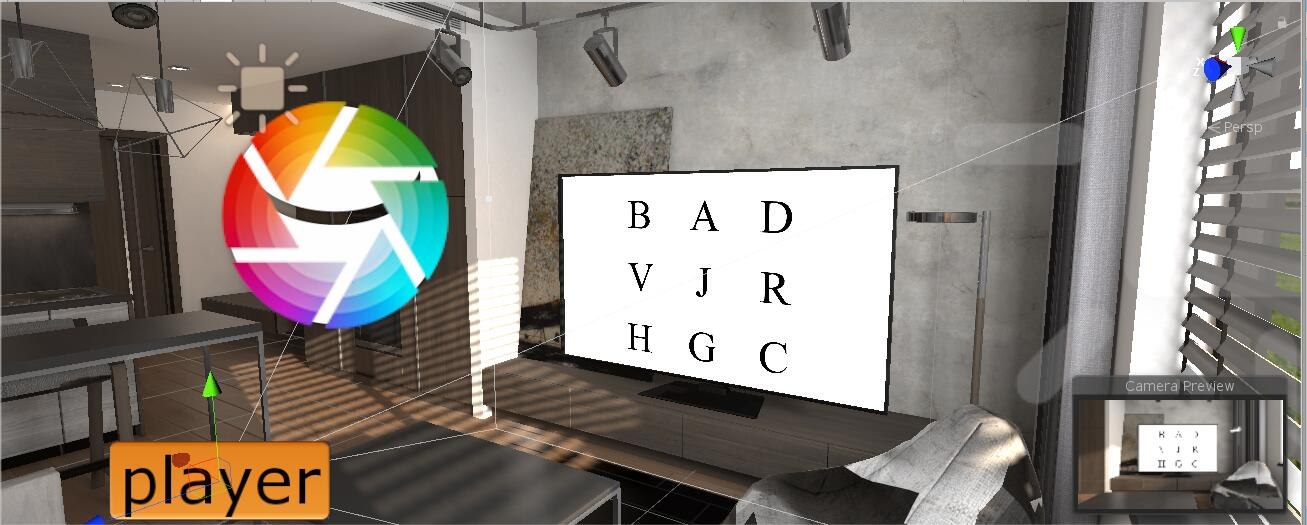
\includegraphics[width=6.0in]{aaafiles/environments_b}
%   \caption{Experiment setup, a visual-searching task was played on TV.}
% \end{teaserfigure}

% Processes all of the front-end information and starts the body of the work.
\maketitle

\section{Introduction}

% 自1968年$, $Ivan Sutherland 与学生 Bob Sproull 创造出第一个虚拟现实及增强现实头戴式显示器系统:达摩克利斯之剑以来 \cite{sutherland1968head}$, $人们对于虚拟现实技术的探索就不曾停歇。近年来$, $一些如HTC VIVE \footnote {\leftidx {^1} https://www.vive.com/us/ }和Oculus Rift \footnote {\leftidx {^2} https://www.oculus.com/}等消费级头戴式虚拟现实设备开始走入寻常百姓家$, $这得益于计算机图形学及相关虚拟现实技术的发展。一方面$, $这使得更多人能够体会“身临其境”的奇妙感觉$, $另一方面$, $许多在过去因为软硬件条件限制而无法解决的问题如今重新回到了人们的视野当中$, $而“有没有办法能够调控用户在虚拟现实环境中的时间感知”就是其中非常有意义和价值的问题。

In 1968, Ivan Sutherland, With the help of his students including Bob Sproull, created what was widely considered to be the first head-mounted (HMD) display system applied to immersive simulation: the sword of Damocles \cite{sutherland1968head}. Since then, researchers have started their continuous exploration of virtual reality (VR) technology. Thanks to the development of computer graphics and VR technology, some VR products for consumers such as HTC VIVE \footnote[1]{https://www.vive.com/us/}  and Oculus Rift \footnote[2]{https://www.oculus.com/} began to be better known. For one thing, it benefits more people by bringing them the experience of the wonderful feeling of "being there" \cite{held1992telepresence,sheridan1992musings,barfield1993sense,slater1997framework,draper1998telepresence,bystrom1999conceptual,sanchez2005presence} or "feeling real" \cite{parola2016turning}. For another, many unsolved problems limited by software and hardware get back to public attention, and the answer to this question that "is there a way to control the temporal perception of the user when they are in the IVEs" is exciting.

% 虚拟现实技术能够以假乱真的重要原因之一就是用户在虚拟现实环境中会产生一种被称之为“临境感”的主观感受$, $通常$, $人们所提到的更多是虚拟现实技术的3I特性:“Immersive, Interactive and Imaginative”中的沉浸感 \cite{Burdea:1994:VRT:177812}$, $沉浸感的其中一个广为接受的定义是“Being there” \cite{heeter1992being}$, $人们对于用户在IVEs中的这种感受的定义的争论始终没有一个统一的答案 \cite{ijsselsteijn2000presence,birkenbusch2013concepts,skarbez2016plausibility,darken1999quantitative}。在2009年$, $M. Slater在 \cite{slater2009place} 中对于为什么参与者倾向于对沉浸式虚拟现实系统中描述的情景和事件做出现实的反应这一问题提出了新的观点$, $即这种现实的反应是由两个正交分量构成的:“位置错觉”和“可能性错觉”$, $其中位置错觉强调的是“一个人觉得自己所处的环境是真实的”$, $可能性错觉强调的是“一个人觉得自己面前所发生的事情是真实的”。和传统概念中强调客观技术指标对虚拟环境产生作用的“沉浸感”不同$, $“存在”$, $也即“临境感”更多地体现了用户在虚拟现实场景中的主观体验$, $这其中自然也包括了对于时间的感知。

The characteristics contributing to VR technology to which people often referred are Immersive, Interactive and Imaginative \cite{Burdea:1994:VRT:177812}. However, there is no generally accepted theory of presence \cite{ijsselsteijn2000presence,birkenbusch2013concepts,skarbez2016plausibility,darken1999quantitative}. In 2009, Mel Slater put forward a widely accepted theory of place illusion (PI) and plausibility illusion (Psi) to the question that why participants tend to respond realistically to situations and events portrayed within an immersive VR system. They argue that when both PI and Psi occur, participants will respond realistically to the virtual reality \cite{slater2009place}. Different from influencing factors of "immersion" which address more on the objective technical condition of VR system \cite{bowman2007virtual,slater1999measuring,riva2011intention,slater1997framework}, the user's subjective experience is more concerned in virual environment (VE) when refers to the presence, Which includes the perception of time.


% “控制时间”这一想法在现实世界中看起来好像是天方夜谭$, $但是虚拟现实技术有让人“梦想成真”的潜力。谈及时间的感知$, $光是自然界中最重要的授时因子。\cite {aschoff1965circadian,roenneberg2007human} 授时因子是一些与时间和生物节律相关的外部或环境线索$, $这些线索可以帮助人们确定自身处于一天中的什么时刻或是给流逝的时间做出标定$, $即时间的速度。对于授时因子的研究最早来自时间生物学中有关生物节律的研究$, $Aschoff在其"Circadian Rhythms in Man"一文中将授时因子描述为“在自然条件下$, $一些周期性的环境因素使得生物节律与地球旋转的周期同步(或夹带), $这些因素被称为授时因子” \cite{aschoff1965circadian} 。在2016年$, $Schatzschneider 等人使用了太阳的移动属性作为其实验的授时因子$, $为了评估认知负荷对于时间感知的影响$, $他们还比较了用户在进行空间认知负荷/言语认知负荷/没有相关认知任务的情况。他们在该篇论文中已经证明了在IVEs中$, $可以通过控制太阳的移动等方式来影响人们的时间估计$, $并且在此过程中增加用户的空间和语言认知负荷会使得被试的时间估计明显缩短 \cite{schatzschneider2016turned} 。根据所了解的文献资料$, $这也是第一个单独评估IVEs中这些因素对于时间评估所造成影响的实验$, $并且也比较了这些因素之间的相互影响。

The idea of time controlling seems to be a fantasy in the real world, but VR has the potential to make it possible. In the context of time perception, light is the most important synchronizers of biological rhythms in nature, Which is referred to as zeitgebers \cite{aschoff1965circadian, roenneberg2007human}. Zeitgebers is a term that describes external or environmental cues that function to entrain the human circadian rhythms and synchronizes our biological rhythms to the Earth's 24-hour day-night cycle and 12-month cycle \cite{aschoff1965circadian,pittendrigh1981circadian}. Such cues help people determine what time they are at in the day or to mark the elapsed time, namely the speed of time. The study of zeitgebers derived from the study of biological rhythms in chronobiology. Aschoff concluded that under natural conditions, the circadian period synchronized with (or entrained to) the period of the earth's rotation utilizing periodic factors in the environment, called zeitgebers \cite{aschoff1965circadian}. In 2016, Schatzschneider et al. used various virtual sun movement speeds as zeitgebers for their experiments. They use dual-task studies to test the influences of the cognitive load on time perception and proved that it is feasible to manipulate such zeitgebers to affect time judgments. Moreover, they found that increased spatial and verbal cognitive load resulted in a significant shortening of judged time as well as an interaction with the external zeitgebers \cite{schatzschneider2016turned}. 

% 在现实世界和非沉浸式环境中不乏拥有授时因子的场景$, $其中大多数场景都来源于视频或是电脑游戏 \cite{bruder2014threefolded,tobin2009video}。人们在太过投入时总是会产生一种时间飞逝的感觉 \cite{sanders2010time}$, $而对于这种现象背后的解释也不一而足$, $比如基于注意力机制的相关解释 \cite{block2010cognitive,张义芳2011时间知觉的影响因素研究综述}$, $基于情绪机理的相关阐述 \cite{angrilli1997influence,droit2007emotions}$, $一些研究者从不同的时间估计范式来对这一现象进行解释 \cite{block1997prospective,赵雪2012时距知觉研究综述}$, $也有一些研究者试图从心流理论阐明这一现象 \cite{nakamura2014concept,csikszentmihalyi1997finding}。而在这篇论文中$, $我们探究的问题包括但不限于:如光照强度这种视觉模态信息或时钟声音速度这种声音模态信息能否被用作授时因子从而影响被试在IVEs中的时间感知表现。如果确实可以$, $那么这种授时因子能够多大程度上影响被试的时间感知能力?用户在IVEs中的时间知觉与临境感是否有关系?如果有$, $是什么样的关系?

Scenes with zeitgebers in reality and non-immersive environments are common, many of which are from video or computer games \cite{bruder2014threefolded,tobin2009video}. Moreover, people will always report losing their sense of time passing when having fun \cite{sanders2010time}. Accounting for these situations are various explanations, such as attention-based explanation \cite{block2010cognitive,张义芳2011时间知觉的影响因素研究综述}, emotion-based explanation \cite{angrilli1997influence,droit2007emotions}, different estimation paradigms \cite{block1997prospective,赵雪2012时距知觉研究综述}, flow theory \cite{nakamura2014concept,csikszentmihalyi1997finding} and so on. However, in this paper, We try to figure out whether the visual modal information changed by illumination intensity or the audio modal information generated by the ticking of a clock can be used as zeitgebers to affect the user's time perception in IVEs. If so, how much do these zeitgebers affect user's time perception? Does the user's perception of time in IVEs have a relationship with the sense of presence? If so, What kind of relationship?

% 在本文中$, $我们提出了一个关于时距估计的探索性定性实验$, $在这个实验中$, $我们以不同程度的光照强度和时钟声音速度结合认知负载分别对用户在沉浸式和非沉浸式环境下的时间感知及临境感的影响进行了探究。实验中使用“visual gains”来描述强、中、弱三种程度的光作为视觉模态授时因子$, $还加入“auditory gains”来描述快、中、慢三种速度的时钟声音作为听觉模态授时因子$, $为了探究认知负载的影响$, $以没有视觉搜索任务的情况作为基线$, $采用双任务法分别探究了在有/无视觉搜索任务情况下授时因子对于时距估计和临境感的影响程度$, $结合了主客观测量方法共同探究授时因子和认知负载对时间认知和临境感的关系。目前来看$, $这是首个采用光照或时钟声音结合视觉搜索任务对用户在IVEs中的时间知觉以及临境感的影响进行评估的实验$, $与此同时文中也对这些因素的交叉效应进行了分析。

In this paper, We presented an exploratory qualitative experiment on time estimation, in which we combined cognitive load with illumination intensity or ticking speed of a clock in different levels for users in immersive and non-immersive environments. Thus the effects of zeitgebers and cognitive load on time perception and presence were explored. In the experiment, visual gains were used to describe the three levels of illumination intensity as the visual modal zeitgebers, namely the bright light, the medium light, and the dim light. Auditory gains were used to describe the three levels of ticking speed as the audio modal zeitgebers, namely the quick ticking, the medium ticking, and the slow ticking. To test the effect of cognitive load, We compared conditions with a visual-searching task and a baseline condition without a cognitive task. As we know, this is the first experiment so far to evaluate the influence of users' time perception and presence in IVEs by using illumination intensity or ticking speed of a virtual clock combined with a visual-searching task, and we also compared their interactive effects of these factors.

% 总而言之$, $我们的文章通过分析以下内容而做出了贡献:

% * 以光照强度或时钟声音作为外部授时因子对用户在IVEs中的时间知觉以及临境感的影响以及在非沉浸环境下的区别
% * 以视觉搜索任务作为认知任务结合光照强度或时钟声音等外部授时因子对用户在IVEs中的时间知觉以及临境感的影响以及在非沉浸环境下的区别
% * 结合了主客观测量方法共同探究授时因子和认知负载对时间认知和临境感的关系。
% * 在某种程度上对于调控用户在IVEs中的时间知觉具有启发性和指导意义。
% * 在某种程度上可与真实世界中对于时间知觉的已有结论相互论证更新。

% 文章的剩余结构如下:第二部分会讨论与此工作相关的背景和相关工作;第三部分会描述具体实验;结果会在第四部分进行呈现$, $在第五部分进行讨论;第六部分是文章总结。

All in all, our article made positive contributions by analyzing the following:
\begin{itemize}
\item effects of the illumination intensity or ticking speed as an external zeitgeber on the user's perception of time and presence in IVEs and the difference they show in non-immersive environments,
\item effects of visual-searching cognitive task with multimodal information as zeitgebers on time estimation and presence,
\item feasibility of combining subjective and objective measurement methods to explore the relationship between zeitgebers and cognitive load on temporal perception and presence and
\item implications for regulating the user's perception of time in IVEs.
\end{itemize}

The remaining structure of the article is as follows. Section 2 discusses the background and literatures related to this article. Section 3 describes the experiment in which we evaluate the time estimation in IVEs. The results are presented in Section 4 and discussed in Section 5. Section 6 concludes the article.

% \begin{figure}[ht]
%   \centering
%   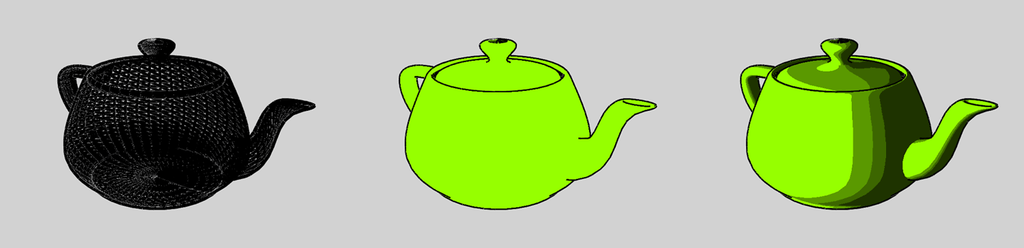
\includegraphics[width=\linewidth]{aaafiles/teapots}
%   \caption{Cel-shaded teapots. Image by Nicolas Sourd [CC-BY-SA-3.0 (http://creativecommons.org/licenses/by-sa/3.0/)], via Wikimedia Commons. (\url{https://goo.gl/5e6tNk}).}
% \end{figure}

% Duis sagittis massa odio, consequat ornare mauris imperdiet blandit. \cite{levoy:2000:TDM} Donec vel pulvinar nisl. Nam pretium vitae risus a consectetur. \cite{sako:2001:SSB, fedkiw:2001:VSO, Jobs95} Vestibulum efficitur auctor mauris. Vestibulum nec orci suscipit, faucibus mauris vel, elementum dolor. Phasellus ornare est id commodo cursus. Lorem ipsum dolor sit amet, consectetur adipiscing elit. Donec iaculis enim urna, vitae tincidunt est dictum id. Suspendisse lobortis justo id enim ornare euismod. Fusce quis turpis rhoncus, laoreet lorem eu$, $porttitor enim. \cite{kartch:2000:ERA, yee:2000:SSA$, $parke:1996:CFA} Etiam eget tempus velit. Duis iaculis id eros et mollis. Pellentesque non magna a massa rhoncus gravida id eget ex. Donec magna risus$, $posuere eu velit sit amet, tincidunt cursus leo. Curabitur non ultricies turpis, at sodales sapien.

\section{BACKGROUND AND RELATED WORK}\label{chap:backgound}

% 在这一部分会对授时因子、认知负载、时间感知和临境感进行统览$, $同时还会讨论在IVEs中$, $授时因子和认知负载对于时间感知和临境感的可能影响$, $系统关系如图\ref{fig:background}.

% \begin{figure}[!htbp]
%     \centering
%     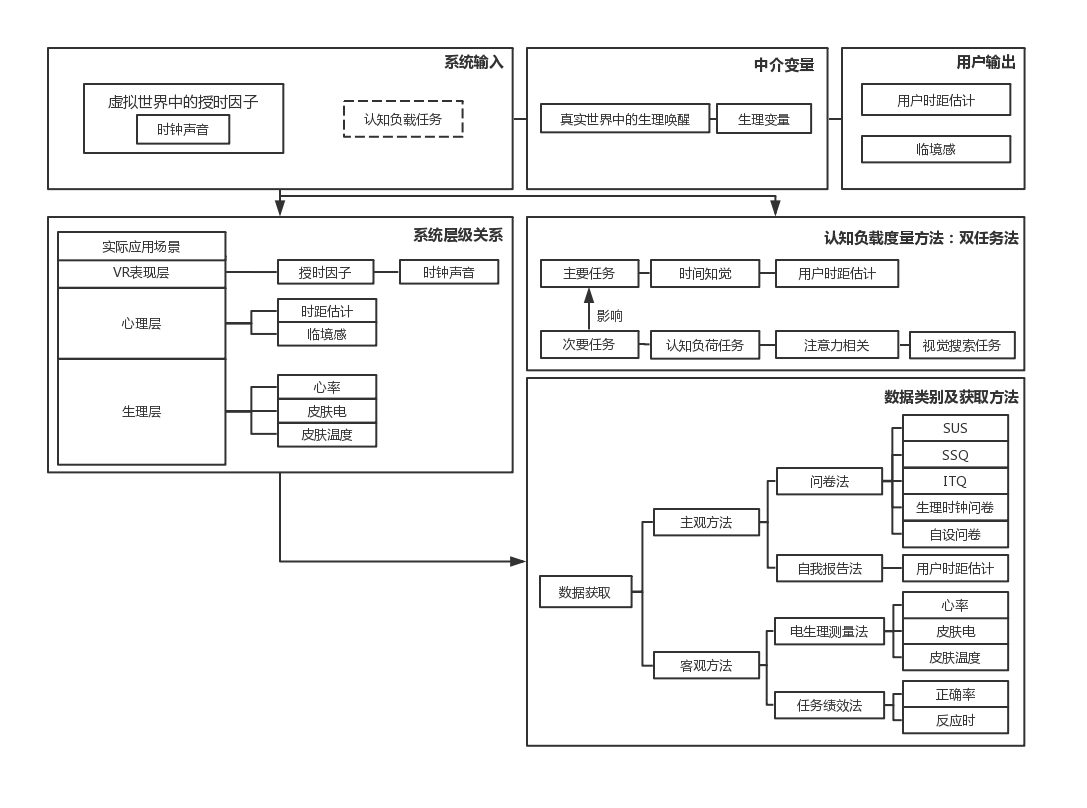
\includegraphics[width=1.00\textwidth]{background}
%     \bicaption{系统关系图}{System Relationship}
%     \label{fig:background}
% \end{figure}

In this part, We will make an overview of zeitgeber, cognitive load, time perception, and presence. Moreover, We discuss the possible influence of zeitgeber and cognitive load on time perception and presence in IVEs. %系统关系如图\ref{fig:background}.

\subsection{Zeitgebers}

% 授时因子一词来源于德语$, $意为“时间授予者”$, $我们首先对其相关的两个概念进行一下区分:

% * 外部授时因子:通常用于指代环境中那些能够对体内生物节律造成影响的环境因素$, $比如光照 \cite{aschoff1965circadian}或社会因子 \cite{ehlers1988social}。
% * 内部授时因子:体内或器官内的组织、时钟模型或与时间相关的认知策略$, $比如SCN \cite{buijs2003circadian}或信息处理模型 \cite{gibbon1984scalar}。

The term zeitgeber originates from German and means "time-giver". First, we differentiate between external and internal zeitgebers:

\begin{itemize}
\item \emph{External (or exogenous) zeitgebers}: usually refer to environmental cues that affect the biological rhythm of the body, such as lighting \cite{aschoff1965circadian} or social cues \cite{ehlers1988social}.
\item \emph{Internal (or endogenous) zeitgebers}: something inside your body or organism, like the suprachiasmatic nucleus or nuclei (SCN) \cite{buijs2003circadian} or different internal-clock models of interval timing like information processing model for example \cite{gibbon1984scalar}.
\end{itemize}

% 生物节律由内部生物钟和外部授时因子共同控制$, $而调整体内的生物钟与外部授时因子相协调的这一过程被称为夹带 \cite{duffy2005entrainment}$, $光和其他环境以及社会因子在夹带过程中发挥着重要的作用。研究表明$, $位于下丘脑的SCN是控制我们昼夜节律的内源性起搏器 \cite{albrecht2003mammalian}$, $即SCN是生物钟所在的位置。以光照为例$, $光会给SCN传递昼夜信息$, $而这一过程会影响松果体中褪黑素的分泌$, $当光较弱时会抑制褪黑素的分泌$, $光较强时则会促进褪黑素的分泌 \cite{duffy2005entrainment}。所以在这个夹带的过程中$, $光使得内部的生物钟与外部世界统一起来$, $还有研究表明体内的一些振荡细胞也具有光感性$, $即我们也许并不需要依赖我们的视觉系统来感知光。

External zeitgebers and internal clock jointly control the biological rhythm, and the process of adjusting the internal clock to coordinate with external zeitgeber is called entrainment \cite{duffy2005entrainment}. Light and other environmental and social zeitgebers play an essential role in entrainment. Studies have shown that SCN located in the hypothalamus is an endogenous pacemaker that controls our circadian rhythm \cite{albrecht2003mammalian}. Light will transmit day and night information to SCN, and this process will affect the secretion of melatonin in the pineal gland. When the light is weak, it will inhibit the secretion of melatonin, While when the light is intense, it will promote the secretion of melatonin \cite{duffy2005entrainment}. So in this entrainment process, light unifies the internal clock with the outside world, and studies have shown that some of the oscillating cells in the body are also photosensitive, that is, We may not need to rely on our visual system to sense light.

% 上面提到了社会授时因子$, $这其实是另外的分类方法 \cite{fleissner20138}:

% * 自然授时因子:与实验室环境不同$, $是由自然产生的时间线索$, $比如晨昏时段的光照变化或者不同的气候条件。
% * 人造授时因子:指的是人为制造的时间线索$, $比如人造光源。
% * 社会授时因子:指的是与其他个体交互的时间线索$, $比如每天的日程安排以及进餐时间。

The social zeitgebers mentioned above is another differentiation \cite{fleissner20138}:

\begin{itemize}
\item \emph{Natural zeitgebers}: unlike the laboratory environment, they are natural time cues, such as changes in light at dawn and dusk or different climatic conditions.
\item \emph{Artificial zeitgebers}: artificial time cues, such as artificial light sources or clocks.
\item \emph{Social zeitgebers}: refers to time clues that interact with other individuals, such as daily schedules and meal times.
\end{itemize}

% 然而$, $研究表明$, $人类的生物钟主要受太阳时间的影响$, $而不是受社交时间的影响。如果没有引起光线变化的行为干预$, $社会线索就不能使人类的生物钟正常运转。近年来,除了使用视觉模态信息如光授时因子\ {roenneberg2007human, duffy2005entrainment},一些研究者开始探索多通道信息等时间估计的影响音乐的节奏\ {pizarro2016s},这些尝试是有价值的对于理解如何操作时间知觉的用户在虚拟现实环境中。

However, studies have shown that the human circadian clock is predominantly entrained by sun time rather than by social time. Social cues cannot entrain the human circadian clock without behavioral intervention which caused light changes \cite{roenneberg2007human}. In recent years, in addition to using visual modal information such as light as zeitgebers \cite{roenneberg2007human, duffy2005entrainment}, some researchers began to explore the influence of multimodal information on time estimation such as the tempo of music \cite{pizarro2016s}. These attempts are valuable for understanding how to manipulate the time perception of users in virtual reality environments.

% 在这篇文章中$, $我们把授时因子一词用于指代人们在外部世界中可以感知到的与时间相关的所有信息$, $而不仅限于生物节律领域内的定义。据此$, $我们提出将外部授时因子根据人的感知觉进一步分为以下类别:

% * 视觉授时因子:外部环境中人们通过观察能够获取到的与时间相关的信息$, $比如环境的明亮程度。
% * 听觉授时因子:外部环境中人们通过聆听能够获取到的与时间相关的信息$, $比如时钟滴答声。
% * 嗅觉授时因子:外部环境中人们通过闻味能够获取到的与时间相关的信息$, $比如熏香。
% * 味觉授时因子:外部环境中人们通过品尝能够获取到的与时间相关的信息$, $比如辛辣。
% * 触觉授时因子:外部环境中人们通过感觉能够获取到的与时间相关的信息$, $比如温度。

In this paper, We apply the term zeitgeber to refer to all time-related information that people can perceive in the external world, not just in the field of biological rhythm. Based on this, We further divide external zeitgebers into the following subcategories according to human's perception:
\begin{itemize}
\item \emph{Visual zeitgebers}: time-related information that people can obtain by observing the environment, such as the brightness of the environment.
\item \emph{Auditory zeitgebers}: auditory information which indicates the elapse of time, like ticking of a clock.
\item \emph{Olfactory zeitgebers}: information of olfactory modal which affects time perception, such as incense.
\item \emph{Gustatory zeitgebers}: the taste which influences time perception when tasting the flavor of it, like spicy.
\item \emph{Tactile zeitgebers}: refers to the haptic information that people perceive in the environment and has effect on time perceptin, such as temperature.
\end{itemize}
% 人们在日常生活中所能感受到的最直观的时间信息来源是视觉和听觉授时因子$, $如一天中的明亮变化 \cite{duffy2005entrainment,pittendrigh1981circadian,fleissner20138,lopez2006light,aschoff1965circadian} 以及所听到的时间声响 \cite{noulhiane2007emotional}$, $触觉授时因子最主要的表现形式便是温度$, $而温度也是重要的生物节律影响因子 \cite{lopez2006light,aschoff1965circadian}。至于嗅觉和味觉授时因子对于时间感知的影响可能并不是那么直接$, $即它们可能通过影响人的生理唤醒或情绪效价等方式来对人们的时间感知造成影响 \cite{angrilli1997influence,burle2001dissociation,droit2007emotions}。
% 在这篇文章中$, $我们主要关注的是视觉和听觉授时因子$, $具体而言即场景光源的明亮程度及时钟滴答声的速度$, $并且假设光照强度弱及时钟滴答声快的情况下人们会认为时间过得更快$, $即主观时距估计值大于客观时距。同时预计视觉和听觉授时因子不会对被试临境感造成影响。

The most intuitive source of time information that people can feel in their daily lives is visual and auditory zeitgebers, such as the light changes of the day \cite{duffy2005entrainment, pittendrigh1981circadian, fleissner20138, lopez2006light, aschoff1965circadian} and the sound which indicates the elapse of time \cite{noulhiane2007emotional}, the most important form of tactile zeitgebers is temperature, Which has an important effect on biological rhythm \cite{lopez2006light, aschoff1965circadian}. The effects of olfactory and gustatory zeitgebers on time perception may not be so direct, that is, they may affect people's perception of time by affecting people's physiological arousal or affective valence \cite{angrilli1997influence,burle2001dissociation,droit2007emotions}.

In this article, We focus on the visual and auditory zeitgebers, specifically, the intensity of the light and the speed of clock ticking, and assume that time flies under the condition of the dim light or the quick ticking of the clock%, that is, the subjective time interval estimate is greater than the actual time interval%
. At the same time, visual and auditory zeitgebers are not expected to affect the sense of presence.

\subsection{Cognitive Load}

% 当提到认知负载的时候$, $指的是信息处理过程中所需的注意力或工作记忆资源 \cite{block1997prospective}$, $其中前瞻性时间估计范式需要更多的注意力资源$, $而回溯性时间估计范式需要更多的工作记忆资源 \cite{block2010cognitive}(有关时间估计范式的详细内容见 \ref{sec:timepeception})。

When referring to cognitive load, it refers to the attention or working memory resources required in the information processing process\cite{block1997prospective}, where the prospective time estimation paradigm requires more attention resources, while the retrospective time estimation paradigm requires more working memory resources \cite{block2010cognitive} (for detailed information about the time estimation paradigm, see \ref{sec:timeperception}).

% 在本篇文章中$, $并没有如 \cite{schatzschneider2016turned}一样选择与工作记忆资源相关的认知任务$, $而是选择了与注意力资源更相关的视觉搜索任务作为认知任务。这样的选择出于以下考虑:此次实验将会采用前瞻性时间估计范式$, $即提前告知被试需要在任务结束后反馈给主试时距估计值$, $选择与注意力资源更相关的视觉搜索任务作为认知任务不仅因为每位被试需要进行多组实验$, $回溯性时间估计范式不适用于该种情况 \cite{block1997prospective}$, $也因为无论是前瞻性还是回溯性时间估计范式$, $其时距估计值相比客观时距都偏低$, $但是前者的时距估计值略微大于后者$, $即前瞻性时间估计范式的时距估计值更加准确 \cite{杨珍2006时距估计范式与方法效应的实验研究}$, $本实验期望通过使用与注意力资源更加相关的认知任务对被试的时距感知造成更大的影响。具体而言$, $在此次实验的双任务法背景下(与双任务法有关的详细内容见下文), $根据有限注意资源理论 \cite{kahneman1973attention,navon1979economy,wickens1980processing}$, $次级认知任务的有无及难度都会影响主要时距估计任务的表现。

In this article, instead of selecting cognitive tasks related to working memory resources like \cite{schatzschneider2016turned}, a visual-searching task more relevant to attention resources is selected as the cognitive task. This experiment will use a prospective time estimation paradigm that informs the participants in advance that they need to report the elapsed time at the end of each group of experiment. The reason for choosing the visual-searching task based on attention resources as the cognitive task is as follows: per participant needs to perform multiple groups of experiments, so the retrospective time estimation paradigm is not suitable for this case \cite{block1997prospective}. Moreover, prospective time estimation paradigm is more accurate than retrospective time estimation \cite{杨珍2006时距估计范式与方法效应的实验研究} (see \ref{sec:timeperception} for more details). In this experiment, we expect to have a more significant impact on the time estimation of participants by using cognitive tasks that require more attention resources. Specifically, through using the dual-task method (see \ref{sec:methods} for more details), the difficulty of secondary cognitive tasks will affect the performance of the primary task of time estimation according to the attentional resource theories \cite{kahneman1973attention,navon1979economy, Wickens1980processing}.

% 在本实验中$, $规定有认知任务的情况为\emph{高认知负载}$, $无认知任务的情况为\emph{低认知负载}$, $则预计\emph{高认知负载}会弱化视觉或听觉授时因子对于被试时距估计的影响$, $且最终主观时距估计值低于客观时距。此外$, $预计在两种不同认知负载情况下$, $被试的皮肤温度等生理指标及临境感存在差异。

In this experiment, the condition with cognitive tasks is \emph{high cognitive load}, and the case of non-cognitive tasks is \emph{low cognitive load}. We expected that the condition of \emph{high cognitive load} will weaken the influence of visual or auditory zeitgeber on the time interval estimation, and the reported estimation of time will lower than the actual time interval. Besides, we assume that there are differences in physiological variables such as skin temperature and the sense of presence under the two different cognitive load conditions.

\subsection{Time Perception}\label{sec:timeperception}

% 时间知觉(time perception)指个体对直接作用于感觉器官的客观时间的持续性和顺序性的反映 \cite{宋其争2004时间认知的理论模型探析}。其分类包括时序知觉和时距知觉$, $前者主要指的是在一段时间中人们不仅能感受到事件发生的先后顺序也能联系它们之间的关系 \cite{张义芳2011时间知觉的影响因素研究综述}$, $而后者是时距认知的一部分$, $指两个连续时间之间的时间间隔或某一事件持续时间的时间段 \cite{赵雪2012时距知觉研究综述}。研究发现$, $时距加工存在着两种认知机制:自动加工和控制加工。短时距的加工方式通常为自动加工$, $其依赖感觉通道$, $不受注意、生理唤醒等因素的影响$, $而长时距的加工方式主要为控制加工$, $受到注意资源、工作记忆资源及生理唤醒等因素的影响 \cite{张志杰2006不同时距加工机制的比较}。

Time perception refers to the individual's reflection of the duration and order of time flows acting on sensory organs directly. Its classification includes temporal order perception and duration perception \cite{宋其争2004时间认知的理论模型探析}. The former mainly refers to a period in which people can not only feel the sequence of events but also relate the temporal relationship between them \cite{张义芳2011时间知觉的影响因素研究综述}. While the latter is part of time interval cognition, referring to the time interval between two consecutive times or the duration of an event \cite{赵雪2012时距知觉研究综述}. The study found that there are two cognitive mechanisms for time estimation which are triggered by arousal levels: a controlled-attention mechanism for low arousal and an automatic mechanism for high arousal. For the short duration, of which the mechanism is usually the  automatic mechanism, which related to motivational-survival systems and is not affected by attention, physiological arousal and so on. While for the long duration, the mechanism of it is the controlled-attention mechanism, which is affected by attention resources, working memory resources and physiological arousal \cite{张志杰2006不同时距加工机制的比较}.

% 对于时距认知的影响因素有很多 \cite{angrilli1997influence}$, $如前瞻性时距估计显著大于回溯性时间估计$, $由于二者时距估计都倾向于低估$, $因此前瞻性时距估计一般比回溯性时距估计更准确 \cite{block1997prospective,buhusi2005makes,gibbon1997toward,赵雪2012时距知觉研究综述,杨珍2006时距估计范式与方法效应的实验研究};高认知负载情况下会有一种时光飞逝的感觉 \cite{gibbon1984scalar};生理唤醒程度的提高会使得体内生物钟计数加快从而让人感觉过了更长的时间 \cite{angrilli1997influence,burle2001dissociation};在相同生理唤醒程度下$, $使人情绪效价偏向负面的刺激会让人有更加“难熬”的感觉 \cite{droit2007emotions,noulhiane2007emotional};而人们在“忘我”地沉浸在游戏世界中时也会忽略时间的流逝 \cite{sanders2010time,schatzschneider2016turned,jancke2009virtual} 等等。

Many factors affecting duration perception, such as different time estimation paradigm, particularly, duration estimation of prospective paradigm slightly greater than retrospective one, and due to the reason that both of them tend to underestimate the actual time, so prospective paradigm is more accurate than retrospective paradigm \cite{block1997prospective,buhusi2005makes,gibbon1997toward,赵雪2012时距知觉研究综述,杨珍2006时距估计范式与方法效应的实验研究}. People always forget about time elapsing under the condition of high cognitive load \cite{gibbon1984scalar}. The increase in physiological arousal will make the internal-clock of body count faster and make people feel time flies \cite{angrilli1997influence,burle2001dissociation}. Under the same level of arousal, people will judge negative stimuli longer than positive ones \cite{droit2007emotions, noulhiane2007emotional}. Moreover, people will ignore the elapsion of time when they devote themselves to the game world \cite{sanders2010time, schatzschneider2016turned, jancke2009virtual} and so on.

% 在本文中$, $我们主要关注的是被试在无特殊刺激的 IVEs 中对于一段较长时距的估计是否会受到认知负载的影响$, $并且假设被试的时距估计值在高负载情况下比低负载情况更短。

In this paper, We mainly focus on whether the estimation of a long time interval in a peaceful IVEs will be affected by cognitive load, and assume that the estimation of the participants is shorter under \emph{high cognitive load} than under \emph{low cognitive load}.

\subsection{Presence}

% 当提及虚拟现实$, $比起临境感(presence), $人们往往更熟悉沉浸感(immersion), $这两者之间既有密切的联系$, $又有所区别。

Immersion is often more familiar than presence when it comes to virtual reality, which is both closely related and different.

% 沉浸感的一个广为接受的定义是“它指的是虚拟现实系统所能提供的感官逼真度” \cite{meehan2002physiological}$, $它强调的更多的是系统的客观属性对虚拟环境产生的作用$, $如图像逼真度 \cite{welch1996effects}$, $帧率 \cite{chan1996effects}以及动态阴影 \cite{slater1995influence}等。

A widely accepted definition of immersion is \emph{it refers to the objective level of sensory fidelity a VR system provides} \cite{meehan2002physiological}, Which emphasizes more about the role of the attributes of the system in the virtual environment. Such as image fidelity \cite{welch1996effects}, frame rate \cite{chan1996effects} and dynamic shadow \cite{slater1995influence}.

% 而临境感则更多从用户主观感受出发$, $强调用户“身处虚拟环境中$, $而不是肉体所处的物理环境”的体验 \cite{witmer1998measuring}。2009 年$, $Mel Slater在 \cite{slater2009place} 中提出了新的表述临境感的方式——位置性错觉(place illusion$, $pI)和可能性错觉(plausibility illusion$, $pSi)。其中前者强调的是用户“认为自己所处的环境是真实的”这一感觉$, $后者强调的是用户“认为自己面前所发生的事情是真实的”这一感觉。如此而言$, $沉浸感即是临境感的基础$, $它限制了位置性错觉所能达到的极限 \cite{Skarbez2017A}。

The sense of presence is more from the user's subjective feelings, emphasizing the experience of the users' \emph{subjective experience of being in one place or environment, even when one is physically situated in another} \cite{witmer1998measuring}. In 2009, Mel Slater proposed a new way of expressing immersion in \cite{slater2009place}: place illusion (PI) and plausibility illusion (PSi). The former emphasizes \emph{the qualia of having a sensation of being in a real place}, While the latter emphasizes \emph{the illusion that the scenario being depicted is actually occurring}. In this sense, immersion is the basis of the sense of immersion, which limits the PI.

% 事实上$, $沉浸感和临境感都可归为“存在”问题$, $而在“存在”研究领域中$, $一方面$, $由于研究者们侧重的不同$, $除了已经提到的沉浸感(immersion)和临境感(presence)之外$, $诸如参与感(involvement)\cite{witmer1998measuring}$, $空间存在(spatial presence)\cite{Hartmann2015Spatial}和唤醒度(evoked reality)\cite{Pillai2013Achieving}等定义如雨后春笋般出现$, $这也导致了研究者们对于用户在IVEs中的这种感受的定义的争论始终没有一个统一的答案 \cite{ijsselsteijn2000presence,birkenbusch2013concepts,skarbez2016plausibility,darken1999quantitative};另一方面$, $正是由于没有统一的存在感定义以及存在感的测量条件不一等原因$, $至今也没有一个公认的普适性较好的存在感测量方法 \cite{inbook}。

In fact, both immersion and presence can be classified into the same research field of presence research. On the one hand, because of the different focus of the researchers, in addition to the immersion and presence mentioned previously, there are various other related definitions, like involvement \cite{witmer1998measuring}, spatial presence \cite{Hartmann2015Spatial}, evoked reality \cite{Pillai2013Achieving} and so on, which has led to a consistent debate on the definition of the user's perception of this feeling in IVEs \cite{ijsselsteijn2000presence,birkenbusch2013concepts,skarbez2016plausibility,darken1999quantitative}. On the other hand, due to the reason that there is no unified definition of presence, and the measurement conditions of it are not equal, so far there is no recognized universal presence measurement method \cite{birkenbusch2013concepts}.

% 临境感的量化方法大致可分为两类$, $一类为主观测量方法$, $其包括问卷法 \cite{witmer1998measuring,Catena00usingpresence,nakamura2014concept,Schubert01theexperience}$, $访谈法 \cite{Seligman00positivepsychology:}和体验度量法 \cite{Zhang2017Spatial}等方法;另一类为客观测量方法$, $包括任务绩效法 \cite{Schloerb1995A}和行为测量法 \cite{ijsselsteijn2000presence}等。主观测量方法中如问卷法具有易于使用 \cite{kuschel2007presence}$, $不会打断用户在IVEs中的体验 \cite{ijsselsteijn2000presence,inbook,Wissmath2010Measuring}等优点$, $但有研究者指出问卷法所测量的是“沉浸后”的状态$, $并不是处于沉浸的状态$, $所以问卷法有可能更多测量了系统的属性而不是临境感本身 \cite{steuer1992defining,witmer1998measuring}。而客观测量方法中如生理物理指标法具有不会受到被试先前经历所影响 $, $不需要被试投注精力和不会干预被试的沉浸体验等优点$, $但其被诟病的点在于引起生理指标变化的原因并不一定是临境感本身而可能是外部无关刺激 \cite{van2004measuring}$, $客观测量方法得到的结果与临境感之间的关系也并不是那么的明确 \cite{Wissmath2010Measuring,kim1997telepresence}。

The quantitative methods of immersion can be divided into two categories, one is subjective measurement method, which includes questionnaire \cite{witmer1998measuring, Catena00usingpresence, nakamura2014concept, Schubert01theexperience}, interview \cite{Seligman00positivepsychology:}, quality of experience(QoE) \cite {Zhang2017Spatial} and other methods. The other is objective measurement methods, including task performance \cite{Schloerb1995A} and behavior measurement \cite{ijsselsteijn2000presence}. The advantages of subjective methods are easy to use \cite{kuschel2007presence} and they will not interrupt the user's experience in IVEs \cite{ijsselsteijn2000presence, inbook, Wissmath2010Measuring}. However, some researchers argued that the questionnaire method measures the state of "post-immersive" but not the immersive state so that the questionnaire method may measure the properties of the system more than presence per se \cite{steuer1992defining, witmer1998measuring}. Moreover, the objective measurement method, such as the physiological variables analysis method, has the advantages of not being affected by the previous experience of the subject, independent from the subject's attention and will not interfere with the experience of the subject in IVEs. However, a drawback of the objective measure method is that the collection of its data can be intrusive, which means the reason of the change of physiological variables may be irrelevant external stimuli but not the sense of presence per se \cite{van2004measuring}. Furthermore, the relationship between presence and the data obtained by objective measurement methods remains uncertain \cite{Wissmath2010Measuring,kim1997telepresence}.

% 基于以上讨论$, $在此次实验中$, $我们结合了主观测量方法中的问卷法和自我报告法以及客观测量方法中的生理测量法和任务绩效法共同对授时因子及认知负载对于临境感的影响。具体而言$, $预期被试在不同光照强度或时钟声音速度条件下临境感存在差异$, $且有认知任务情况下的临境感强于无认知任务情况。

Based on the discussion above, in this experiment, we combined the questionnaire method and self-report method as the subjective measurement method and the physiological measurement method and task performance method as the objective measurement method to jointly explain the effects of zeitgebers and cognitive load on the sense of presence. In this scope, we assume that the participants will have a different sense of presence under different level of intensity of the light or ticking of the clock, and the perceived presence with the cognitive task was "stronger" than that without the cognitive task.

\section{EXPERIMENT}

% 在这一部分对采用的探索性定性实验进行描述$, $在这个实验中$, $以不同程度的光照强度和时钟声音结合认知负载分别对用户在沉浸式和非沉浸式环境下的时间感知及临境感的影响进行了探究。实验中使用“visual gains”来描述光视觉模态授时因子$, $使用“audio gains”来描述时钟声音听觉模态授时因子$, $引入视觉搜索任务探究认知负载和授时因子的交叉影响$, $采用双任务法分别探究了在有/无视觉搜索任务情况下授时因子对于时距估计和临境感的影响程度$, $结合了主客观测量方法共同探究授时因子和认知负载对时间认知和临境感的关系。

In this section, we described the experiment in which we analyzed the interactive influences of different external zeitgebers combined with a visual-searching cognitive task on time estimation and presence in IVEs. In the experiment, we amplified and compressed the zeitgebers through \emph{visual gains} and \emph{audio gains}, which represent light intensity and speed of ticking sound separately. Besides, we explored the relationship between cognitive load on time estimation and presence by combining subjective and objective measurements.

\subsection{Participants}

% 我们的实验共分为视觉组和听觉组两个组别$, $共招募了 43 名被试$, $其中 22 名被试(11 名女性$, $11 名男性$, $年龄范围是 18-27$, $M = 20.1363)参与的是视觉组实验$, $其余 21 名被试(11 名女性$, $10 名男性$, $年龄范围是 19-22$, $M = 20.2857)参与的是听觉组实验。所有的被试均为电子科技大学的在校本科生/研究生$, $每一位被试会拿到80¥的被试费。

We recruited 46 participants for our experiment and divided them into the visual group and the auditory group. Among them, 22 subjects (11 female, 11 male, ages 18 - 27, M = 20.1636) participated in In the visual group experiment, the remaining 24 subjects (11 female, 13 male, ages 19 - 22, M = 20.3333) participated in the auditory group experiment. All the participants were undergraduate/graduate students at the University of Electronic Science and Technology of China. All of our participants obtained 80 CNY for compensation.

% 对于视觉组实验的被试$, $有 12 名被试先前有 HMDs 的使用经验;其中有 1 名为左利手$, $ 21 名为右利手;所有被试在观察环境并调整HMD后没有存在模糊的情况$, $有 17 名被试佩戴了近视眼镜参与了实验;所有被试都具有正常/矫正听力;没有被试存在平衡障碍或双目视觉障碍。对于听觉组实验的被试$, $有 10 名被试先前有 HMDs 的使用经验;21 名被试均为右利手;所有被试在观察环境并调整HMD后没有存在模糊的情况$, $有 16 名被试佩戴了近视眼镜参与了实验;所有被试都具有正常/矫正听力;没有被试存在平衡障碍或双目视觉障碍。

For the visual group, 12 participants had previously used HMDs, where 21 were right-handed, and the rest were left-handed. There was no blurred vision in all subjects after observing the environment and adjusting HMD. Seventeen participants wore glasses during the experiments. All of our participants had normal hearing. None of our participants reported a disorder of equilibrium or binocular vision disorders. For the auditory group, 12 participants had previously used HMDs, where 24 were right-handed, and no one was left-handed. There was no ambiguity in all subjects after observing the environment and adjusting HMD. Nineteen participants wore glasses during the experiments. All of our participants had normal hearing. None of our participants reported a disorder of equilibrium or binocular vision disorders.

% 每位参与者的时间总长$, $包括资料填写$, $设备佩戴$, $实验前问卷测试$, $实验$, $休息$, $实验后问卷测试和事后情况说明共两个小时。每位被试会进行五组实验$, $其中两组为非沉浸环境$, $三组为沉浸环境$, $每组实验的时长为十分钟左右$, $每组实验结束后会有五分钟左右的休息时间$, $被试还需要在这段时间内填写一份存在感问卷。

% Fig \ref{fig:flowchat} shows the flow chat of our experiment. 
The total length of each participant, including instructions, pre-questionnaires, equipment-wearing, experiment, breaks, post-questionnaires, and debriefing, was two hours. Each participant would conduct five groups of experiments, two of which were non-immersed environments, and the rest were immersive display condition, in which participants needed to wear the HMD. The duration of each group was about ten minutes. After each group of experiments, there was break of five minutes, and we asked participants to fill out a presence questionnaire during this time.


% \begin{figure*}[h]
%       \centering
%       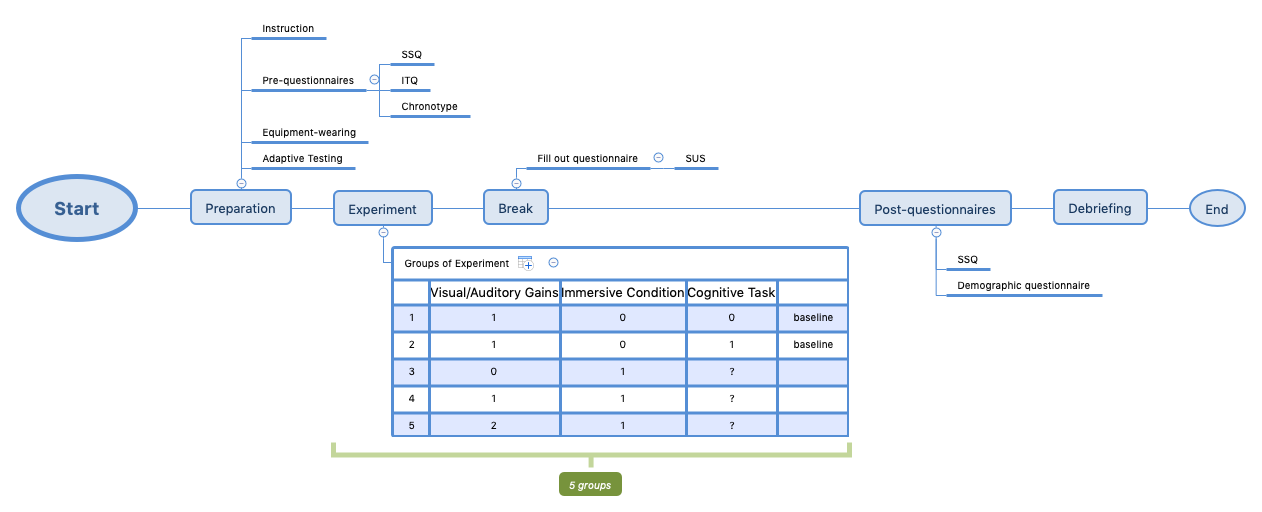
\includegraphics[width=\linewidth]{aaafiles/flowchat.png}
%       \caption{Flow chart of the experiment}
%       \label{fig:flowchat}
% \end{figure*}

\subsection{Material}

% 我们在一个安静的展厅环境进行实验。如图所示{\graph}$, $参与者佩戴一个 HTC VIVE Pro HMD 进行沉浸环境的实验$, $单眼分辨率 1440 × 1600 像素$, $双眼分辨率为 2880 × 1600(这里乘号需要处理), $刷新率为 90 Hz$, $视场角为 110度$, $我们使用 VIVE 定位器以及 SteamVR 追踪技术来进行定位跟踪。我们采用一台工作站进行渲染$, $工作站的处理器为 3.70 GHz Core i7-8700K 处理器$, $24.0GB 主存$, $GeForce GTX 1060 5GB 显卡$, $采用 Unity3D 2018.3.8 对环境进行渲染。我们使用一台工作站作为实验运行平台$, $工作站的处理器为 4.20 GHz Core i7-7700k 处理器$, $16.0GB 主存$, $GeForce GTX 1080Ti 显卡。在实验过程中$, $被试坐在如图N所示的办公椅上{}。被试可以通过移动鼠标(非沉浸环境)或转动头部(沉浸环境)的方式来随意观察环境$, $但我们要求被试在实验进行过程中不能离开座位。

We experimented with one of our showroom environments, which was sealed off during the experiment. As illustrated in Fig. \ref{fig:environments_a}, participants wore an HTC VIVE Pro HMD to carry our the experiment of immersive environment, which provides a resolution of 1440 $\times$ 1600 pixels per eye, and the binocular resolution is 2880 $\times$ 1600 with a refresh rate of 90 Hz and an approximately 110 degrees diagonal field of view. We tracked its position and orientation with SteamVR\texttrademark tracking system. 

\begin{figure}[h]
      \centering
      \includegraphics[width=\linewidth]{aaafiles/environments_a}
      \caption{Experimental setup: photo of a user wearing an HTC VIVE Pro HMD and holding a controller while seated in an office chair}
      \label{fig:environments_a}
\end{figure}

We used a workstation for rendering, whose processor was 3.70 GHz Core i7-8700K processor, 24 GB of main memory and an GeForce GTX 1060 5GB graphics card. The stimuli were rendered with the Unity 3D 2018.3.8 engine. For the experimental platform, we used another workstation, which had a 4.2 GHz Core i7-7700K processor, 16 GB of main memory and GeForce GTX 1080Ti graphics card. During the experiment, the subject sat on the office chair as shown in Fig. \ref{fig:environments_a}. The participants could observe the environment at will by moving the mouse (non-immersive environment) or turning the head (immersive environment), but we asked the participants not to leave their seats during the experiment.

% 在实验过程中会给被试佩戴温柔体温检测仪、皮肤电采集装置 Grove - GSR Sensor 以及心率采集装置 PulseSensor 及小米手环2分别测量被试的皮肤温度$, $皮肤电导以及心率。其中温柔采集装置是浙江智柔科技有限公司 \footnote[1]{http://www.cheroee.com/}出品的 CH-T2 型产品$, $采集精度为 $\pm 0.05 ^{\circ}C$$, $采样频率为5s/次;皮肤电采集装置是 Seeed \footnote[2]{http://wiki.seeedstudio.com/}出品的 Grove - GSR Sensor V1.2 型产品$, $心率采集装置有两个$, $一个是 World Famous Electronics llc \footnote[3]{https://pulsesensor.com/} 出品的 MDL0025 型产品$, $另一个是小米科技有限责任公司 \footnote[4]{https://www.mi.com/us/} 出品的小米手环2。

During the experiment, the subject will wear a flexible temperature patch to measure the skin temperature, a pulseSensor and a MiBand 2 to measure the heart rate of the subject. The flexible temperature patch device is the CH-T2 product produced by Chero Technology Co., Ltd. \footnote[1]{http://www.cheroee.com/}, the temperature measurement accuracy is $\pm 0.05 ^{\circ}C$ and the sampling frequency is 5s/time, and there are two heart rate acquisition devices. One is the MDL0025 product from World Famous Electronics llc \footnote[2]{https://pulsesensor.com/}, and the other is the MiBand 2 product of Xiaomi Technology Co., Ltd.\footnote[3]{https://www.mi.com}.

% 虚拟环境设置在一个现代风格的家居环境中$, $被试将位于客厅中的沙发位置$, $其面前会有一个虚拟屏幕以呈现认知任务$, $如图 \ref{fig:environments_b}所示。在虚拟环境中会有一个百叶窗$, $我们通过在房间外部设置一个方向光来模拟太阳光$, $以 Rotation=(18.64,106.554,0) 角度将光投射到房间内$, $在渲染过程中使用静态渲染技术$, $设置方向光的阴影模式为 Soft Shadows$, $设置物体的着色器为 Standard$, $在每一个单独的实验组中光照强度都为预先设计好的定值$, $光源的其他属性均不变$, $包括阴影在内的所有效果都会预先进行渲染$, $从而使虚拟环境尽可能地真实。为了避免时钟的视觉模型对被试的时距估计造成干扰$, $我们仅在虚拟环境中播放时钟滴答声而不呈现时钟模型$, $通过将时钟声音的多普勒效应置零使其呈现环绕声。

We set the virtual environment in a modern home environment where the participants will be located in the sofa in the living room with a virtual screen in front of them to present cognitive tasks, as shown in the Fig. \ref{fig:environments_b}. There will be a shutter in the virtual environment and we will simulate the sunlight by setting a directional light outside the room, projecting the light into the room at an angle of $Rotation = (18.64, 106.554, 0)$, using \emph{static rendering techniques} during the rendering process. Set the shadow mode of the directional light to \emph{Soft Shadows}. Set the shader of the object to \emph{Standard}. In each experiment group, the light intensity is a pre-designed value, and the other properties of the light source were unchanged, including the shadow. All effects are pre-rendered to make the virtual environment as realistic as possible. In order to avoid the visual model of the clock from interfering with the time interval estimation of the participant, we only play the sound of clock ticking in the virtual environment without presenting the clock model, and the surround sound is rendered by zeroing the \emph{Doppler effect} of the clock sound.

\begin{figure}[h]
      \centering
      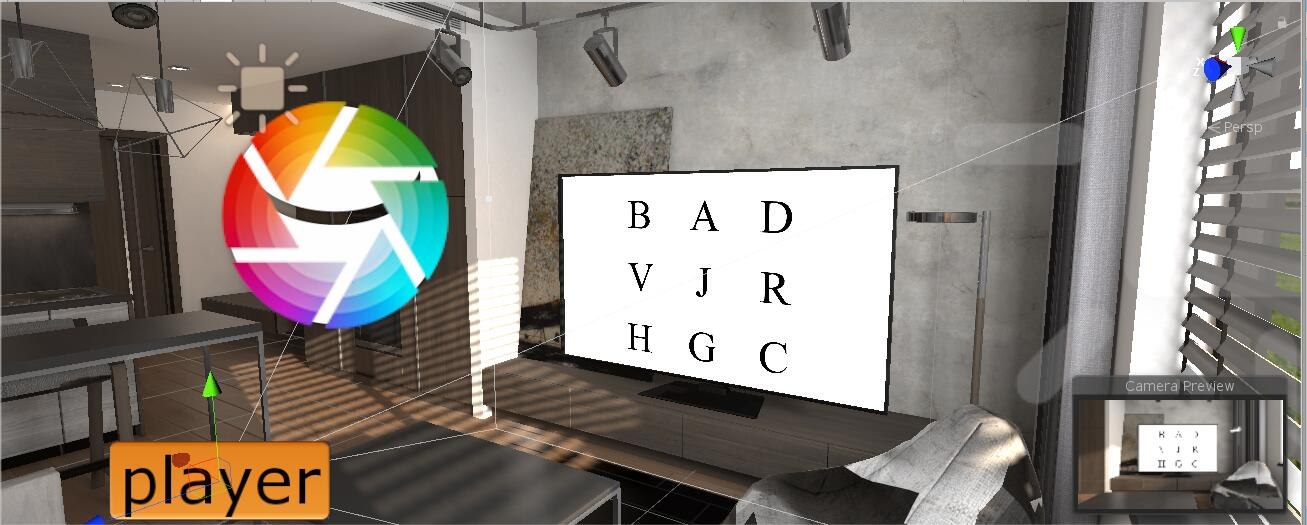
\includegraphics[width=\linewidth]{aaafiles/environments_b}
      \caption{Experimental setup: a virtual living room with a visual-searching task  presented in the TV screen }
      \label{fig:environments_b}
\end{figure}

% \begin{figure*}[H] 
%       \centering 
%       \subfigure[SubfigureCaption]{ 
%       \label{Fig.sub.1} 
%       \includegraphics[width=0.4\textwidth]{aaafiles/environments_a}} 
%       \subfigure[SubfigureCaption]{ 
%       \label{Fig.sub.2} 
%       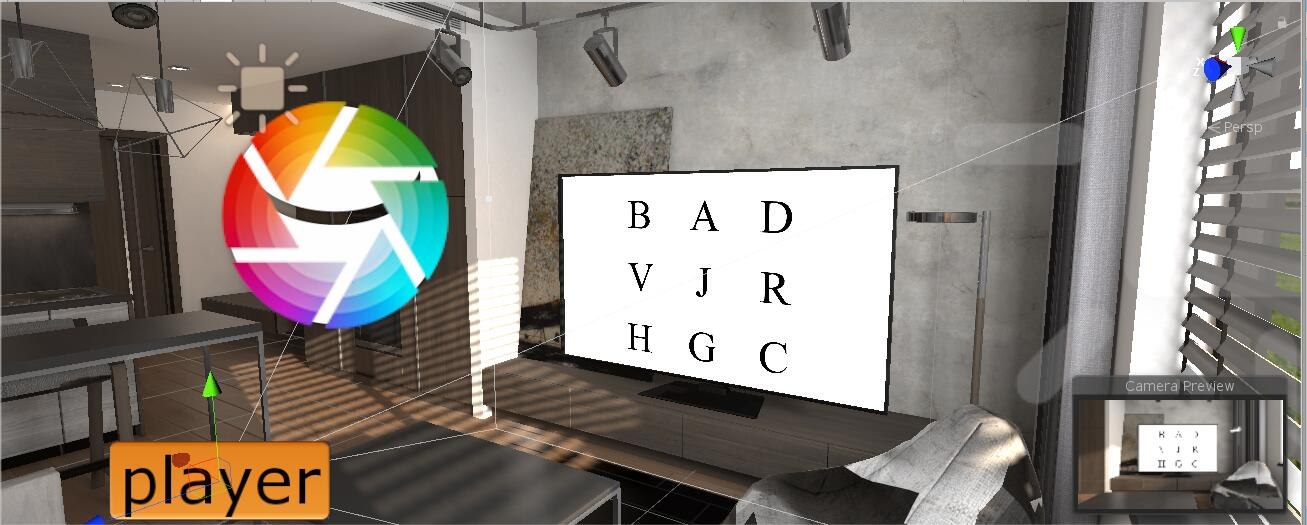
\includegraphics[width=0.4\textwidth]{aaafiles/environments_b}} 
%       \caption{MainfigureCaption} 
%       \label{Fig.lable} 
% \end{figure*}


% \begin{figure}[htbp]   
%       \centering 
%       \subfigure[sin1]
%       {
%         \label{fig:fft:a} 
%         \begin{minipage}[c]{0.5\textwidth} 
%         \centering 
%         \includegraphics[width=6.5cm]{aaafiles/environments_a} 
%         \end{minipage}% 
%       }%注意这个”%”绝对不能省$, $可以试试不打%的效果 
%       \subfigure[sin2]
%       { 
%         \begin{minipage}[c]{0.5\textwidth} 
%         \centering 
%         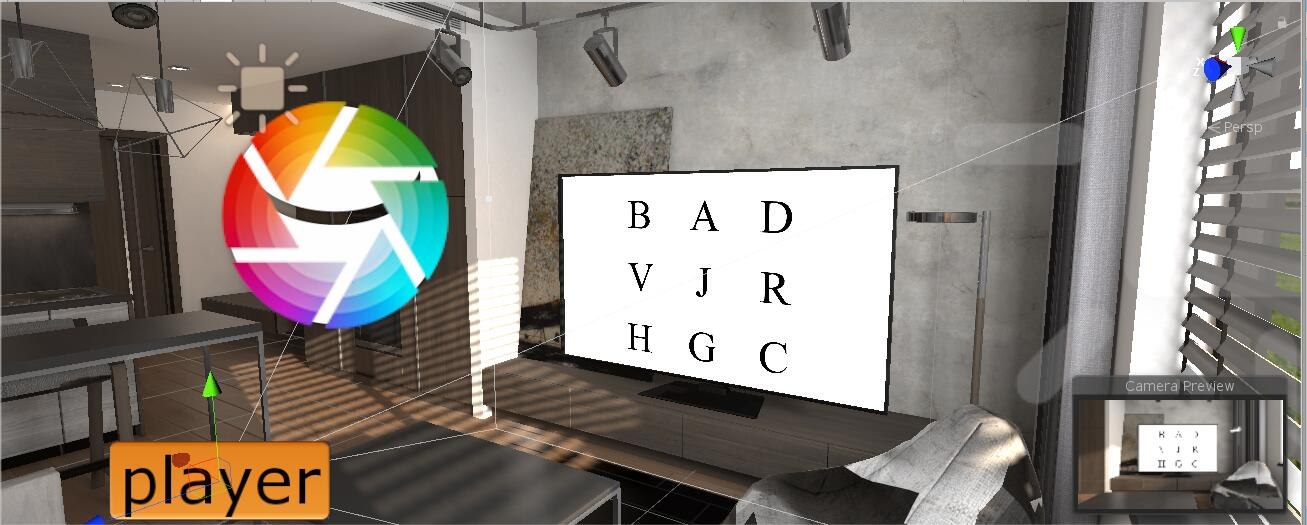
\includegraphics[width=6.5cm]{aaafiles/environments_b} 
%         \end{minipage}
%       }
%         \caption{fft}
%         \label{fig:fft} 
% \end{figure}


% 为了保证被试的临境感$, $主试不会在实验过程中与被试交谈$, $所有的实验讲解都会在正式实验开始前通过文本及口头讲述完成。被试通过按压控制手柄按键完成认知任务$, $在实验过程中被试通过佩戴 HTC VIVE Pro 设备上的 Hi-REs Audio 认证耳机(沉浸环境)或小米入耳式铁圈耳机 QTEJ03JY (非沉浸环境)来聆听虚拟环境中的时钟声音以及减少外界环境对其可能造成的干扰。

In order to maintain the participants' sense of presence in the VE, the experimenter would not have communication with the participants during the experiment. Task instructions would be completed by text and oral narration before the experiment. Participants performed the cognitive task by pressing the trigger or touchpad on a VIVE controller. During the experiment, the participants were wearing Hi-REs Audio certified headphones (immersive environment) on the HTC VIVE Pro device and isten to the sound of the clock in the virtual environment or Mi In-Ear headphones QTEJ03JY (non-immersive environment) to reduce the possible interference to the outside environment.

% 为了探究认知负载对于临境感的影响$, $我们还设置了非沉浸环境下的实验作为 baseline。被试在进行非沉浸条件实验时无需进行头部跟踪。虚拟环境将呈现在一个长虹 60D2P 显示器上$, $其分辨率为 4K(3840 $\times$ 2160), $刷新率为 60Hz$, $被试将佩戴小米入耳式铁圈耳机耳机进行非沉浸条件下的实验。

In order to explore the effect of cognitive load on presence, we also considered a non-immersive display setup with or without a cognitive task as baseline condition. This condition used monoscopic display without head-tracking. The VE would be presented on a Changhong 60D2P display with a resolution of 4K (3840 $\times$ 2160) and a refresh rate of 60Hz. Participants wore in-ear Xiaomi QTEJ03JY headphones for the non-immersive display setup.

\subsection{Methods}\label{sec:methods}

% 有很多对认知负载进行评估的方法$, $包括生理指标法$, $主任务表现法$, $客观调查法和双任务法等 \cite{all9}$, $其中双任务法是其中使用较广的方法之一。双任务法所依据的是注意资源理论 \cite{}$, $它要求被试在进行一项主要任务的同时进行次级任务$, $次级任务所需的注意资源通常与主任务来自统一资源池$, $这意味着当主任务的认知负载增加的同时也会导致次级任务的表现下降 \cite{}。在这篇论文中$, $我们采用双任务法来对认知负载进行评估$, $其主要任务会涉及到在虚拟环境中所经历时距的估计$, $次级任务为视觉搜索任务。

Ways to measure cognitive load include physiological variables measures, primary task performance, opinion surveys, secondary task performance and so on \cite{block2010cognitive}, among which secondary task performance, i.e., dual-task method is one of the most widely used methods. Dual-task method is based on the attention resource theory \cite{kahneman1973attention,navon1979economy%,wickens1980processing%
}, which requires the participant to perform a secondary task while performing a primary task. The attention resources required by the secondary task (i.e., visual-searching task in this paper) usually come from the unified resource pool with the primary task (i.e., estimation of a time interval in the case of this study), which means that when the cognitive load of the primary task increases, the performance of the secondary task decrease.

% 与此同时$, $在实验进行过程中$, $我们还会对被试的心率$, $皮肤电阻及皮肤温度等生理数据进行采集$, $这些生理数据一方面可以对认知负载进行二次评估 \cite{kahneman1973attention}$, $另一方面也可以对临境感进行评估 \cite{wiederhold2001investigation,riva20037,meehan2002physiological}。

At the same time, during the experiment, we will also collect physiological data such as heart rate and skin temperature of the participant. These physiological data can be used to evaluate the cognitive load \cite{kahneman1973attention}, and can also measure the sense of presence \cite{wiederhold2001investigation,riva20037,meehan2002physiological}.

% 在预实验过程中我们发现了很明显的个体差异$, $因此我们决定采用组内比较的方法。因而$, $在挑选被试的过程中$, $我们让被试体验了一个不完整版本的正式实验并要求被试对其在虚拟世界中所经历的时间进行评估$, $规定 ratio 为主观时距与客观时距的比值$, $只选择时距估计能力较好的参与者作为被试(ratio > 0.875)。


We found significant individual differences during the pilot, so we decided to use a within-subjects design for this experiment. Moreover, in the process of recruiting subjects, we asked the participants to experience an incomplete version of the formal experiment and asked the participants to evaluate the time they experienced in the virtual world. We defined \emph{ratio} as the ratio between subjective time interval and real time interval, and only recruited participants with good time duration estimation ability (\emph{ratio} $\in[0.875,1.125]$ ) as subjects .

% 正式实验中共有四种变量$, $分别为光照强度$, $时钟声音速度$, $是否为沉浸环境以及是否有认知任务。其中光照强度共有三个不同的水平$, $i.e., (i)弱光$, $(ii)中等光强$, $及(iii)强光$, $将其标化为收益因子 g_l /in {\frac{1}{3},1,\frac{5}{3}}。对于时钟声音速度共有三个不同的水平$, $i.e., (i)慢速$, $(ii)中速$, $及(iii)快速$, $将其标化为收益因子 g_t /in {\frac{1}{2},1,2}。

There are four variables in the formal experiment, namely the light intensity, the ticking speed of a clock, immersive or non-immersive display setup and whether there is a cognitive task. There are three different levels of light intensity, ie, (i) dim, (ii) medium, and (iii) bright presented as visual gains $g_v \in \left\{0, 1, 2\right\}$ respectively, and there are three different levels of ticking speed, ie, (i) slow, (ii) medium, and (iii) quick, which are presented as the auditory gains $g_a \in \left\{0, 1, 2\right\}$.

% 在正式实验中$, $被试将被随机分到视觉组或听觉组进行实验。无论是视觉组还是听觉组$, $每位被试都需要进行五组实验$, $其中前两组均在非沉浸条件下进行$, $后三组均在沉浸条件下进行。对于前两组实验$, $其变量条件均为中等光强及中速时钟声音$, $i.e., g_l = 1$, $g_t = 1。两组非沉浸实验中有一组有认知任务$, $另一组没有$, $非沉浸条件下的实验顺序会随机产生。非沉浸条件的实验会作为整个实验的基线$, $先进行非沉浸条件的实验也是为了保证被试清楚整个实验的流程。后三组均在沉浸条件下进行$, $对于视觉组$, $被试将以随机顺序进行强光$, $中等光强及弱光条件的实验$, $对于听觉组$, $被试将以随机顺序进行快速$, $中速及慢速时钟声音条件的实验$, $后三组实验中每一组是否有认知任务由被试抽签决定。

In the experiment, we randomly assigned the subjects to the visual or auditory group for experimentation. Whether in the visual group or the auditory group, each subject needs to carry out five groups of experiments, among which the first two groups were carried out in non-immersive display setup, and the rest three groups were all performed under immersive conditions. 

For the first two sets of experiments, the variable conditions were medium light intensity, and medium speed clock sound, i.e., $g_v = 1$, $g_a = 1$. One of the first two groups had cognitive tasks, the other did not, and the sequence of them was random. This non-immersive display setup served as a baseline condition, which also ensured that the subject was clear about the task.

The latter three groups were all performed under immersive conditions. For the visual group, the subjects will perform experiments in bright, medium and dim light intensity in random order. For the auditory group, subjects will perform quick, medium and slow ticking speed randomly. Participants will draw lots to determine whether the last three sets of experiments have cognitive tasks.

% 在实验准备阶段$, $被试需要先填写知情同意书以及观看一份实验指导书$, $以上的工作结束后$, $被试需要先填写一份 Kennedy-Lane simulator sickness questionnaire (SSQ) \cite{kennedy1993simulator}$, $一份 immersive tendencies questionnaire (ITQ) \cite{witmer1998measuring}$, $以及一份 Bio-Time Quiz (BTQ) \cite{Breus:2016}$, $ 而后会给被试佩戴各项生理采集设备(温柔N$, $皮肤电设备N$, $心率采集设备N以及小米手环2)并暂时为被试保管所有的时间设备。在正式实验开始前会根据被试所属的实验组(视觉组或听觉组)让其在所有实验条件下进行适应性测试$, $目的是为了让被试熟悉实验流程以及消除学习效应 \cite{}$, $这一部分的数据不会计入最终的实验结果中。在每一组实验结束后被试都有5分钟的休息时间$, $与此同时被试还需填写一份 Slater-Usoh-Steed questionaires (SUS) \cite{Catena00usingpresence} 问卷。在五组实验做完之后$, $被试需要再次填写 SSQ 问卷$, $除此之外还需填写 SUS 问卷以及自设问卷。

In the preparation stage of the experiment, the participants needed to fill in the informed consent form and received an experimental instruction. After the above work, the participant needed to fill out a Kennedy-Lane simulator sickness questionnaire (SSQ) \cite{kennedy1993simulator}, an immersive tendencies questionnaire (ITQ) \cite{witmer1998measuring}, and a Bio-Time Quiz (BTQ) \cite{Breus:2016}. Then the subject will be wearing various physiological collection equipment (a skin temperature collection device Chero CH-T2 and heart rate acquisition devices, pulseSensor and MiBand 2) and we would keep all the time devices for the subjects during the experiment. Every participant practiced different conditions once at the beginning of the experiment to familiarize it and eliminate the learning effect \cite{莫文2008心理学实验中的各种效应及解决办法}. These trails were excluded from the analysis. At the end of each group of experiments, the participants had a 5-minute break. At the same time, the participants were required to complete a Slater-Usoh-Steed questionnaires (SUS) \cite{Catena00usingpresence} questionnaire. After finishing the five sets of experiments, the participants needed to fill in the SSQ questionnaire again. Besides, the SUS questionnaire as well as a demographic questionnaire.

% 我们采用的是前瞻性时间估计方法 \cite{buhusi2005makes,gibbon1997toward}$, $即被试从开始就知道他们在最后需要给主试提供时距估计值$, $原因如下 \cite{block1997prospective}:
% 前瞻性时间估计方法适用于多次重复试验;
% 前瞻性时间估计方法相较于回溯性估计方法其时距估计更加准确;
% 其更多与注意力资源相关而不是与工作记忆资源相关。
% 得益于前人对于单组实验时距的探索 \cite{schatzschneider2016turned}$, $我们将单组实验时长随机设置为600-650s之间$, $并且告诉被试每次试验时长可能会相差很大由此确保被试并不知道每组实验的具体时长。被试所知的时间信息只有整体实验时间一共是两个小时左右$, $并且他在实验结束之前也不知道一共会进行多少组实验。每组实验都会经历黑屏-实验-黑屏三个阶段$, $在每组实验结束后$, $被试需要马上告知主试在两次黑屏之间共经历了多长时间(需要精确到x分x秒)。

We used a prospective design \cite{buhusi2005makes,gibbon1997toward}, that is, the participants knew from the beginning that they needed to report the time-interval estimation at the end of each experiment. The reasons were as follows \cite{block1997prospective}: 

\begin{itemize}
\item the prospective paradigm applies to repeated experiments, 
\item it is more accurate than the retrospective paradigm, 
\item and it needed more attentional resources than working memory resources. 
\end{itemize}

We draw on the exploration of predecessors on the time interval of each experiment \cite{schatzschneider2016turned}, and randomly set the length of the single experiment to 600-650s and told the participants that the length of each test might vary greatly, thus ensuring that the subjects did not know the specific duration of each set of experiment. The context information known to the participants was only about two hours in total, and they did not know how many experiments would be performed before the end of the whole experiment. Each group of experiments will go through three stages of black screen - experiment - black screen. After each group of experiments, the subjects need to immediately report to us how long it has been between the two black screens by specifying seconds.


To analyze the influence of cognitive load on time estimation and presence when manipulating the visual or auditory zeitgebers, we used a visual-searching task, which was a task with a high requirement for attention resources. Subjects needed to judge whether the visual-searching target appears during each trial and respond by using the VIVE controller. Participants were instructed to perform the task as well as possible.% We recorded all the reaction times and judgment results during the experiment and classified the judgment results as true positives, true negatives, false positives, and false negatives.

\subsection*{Visual-searching Task}

Visual-searching is a classic paradigm used by cognitive psychologists to study attention distribution in complex fields of view. Typical visual-searching tasks require participants to remember the search target and respond accordingly to the presence of targets in the field of view. The visual-searching task used in this experiment consists of multiple trials, each of which undergoes a three-step process of a reticle - character - letters matrix, as illustrated in Fig. \ref{fig:matrix}, and the task was presented on the TV of the living room in VE (see Fig. \ref{fig:environments_b}). The crosshair was to control the subject's attention range, %\cite{}%
and we selected the letters matrix randomly from all the preset matrices with the same probability of occurrence. We instructed participants to press the trigger on the VIVE controller (mouse left in the non-immersive environment) when they found the target character in the letters matrix,  otherwise press the pad button on the controller (right mouse button in the non-immersive environment). There are 144 trails, 24 trails count as one block, and there are six blocks in each group of experiments. At first, the environment is completely black (the first black screen mentioned above) when participant wore the HMD, and he could press any button to start the experiment. In groups with cognitive task, a countdown of six seconds will be displayed on the TV before the visual-searching task, and then the trail will be continuously displayed. There will be about 17.4s break after finishing each block. The presentation time of each reticle, target letter and alphabet matrix is about 1 s, 1s, and 0.4s respectively. The subject had about 1.4s to press the corresponding button after the appearance of the current letter matrix and before the appearance of the next centroid. After the last break of one group of experiment, the environment would go black again (which meant the end of one group of experiment).

\begin{figure}[h]
      \centering
      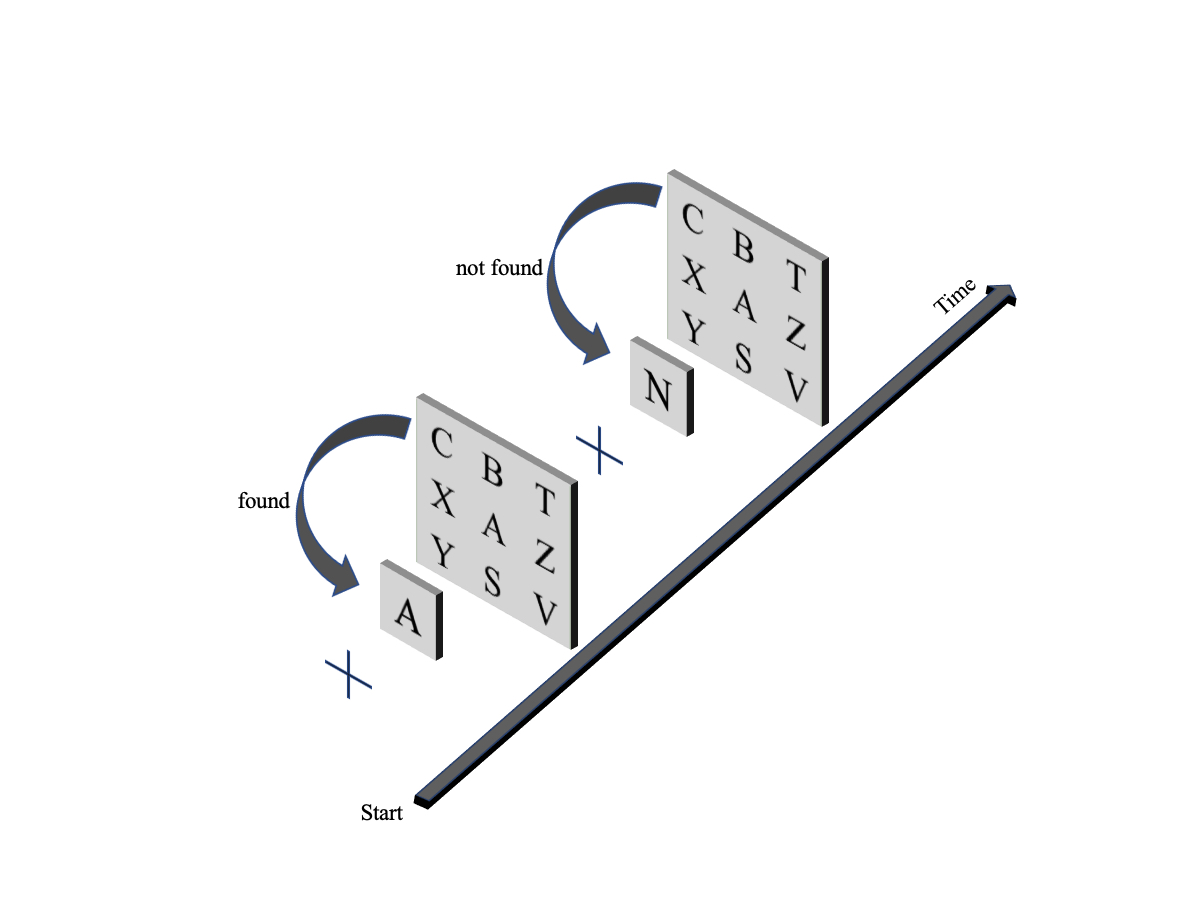
\includegraphics[width=\linewidth]{aaafiles/matrix}
      \caption{Dscription of visual-searching task}
      \label{fig:matrix}
\end{figure}

\subsection*{Hypothesis}

According to the existing literature, we expected that time interval estimation and sence of presence would change under different zeitgeber and cognitive load, and we define temporal judgment deviation equals to estimation of time - Real time duration. Hence, we made the following hypothesis:

\begin{enumerate}[H 1]
\item Mean temporal judgment deviation differs between the three visual gain conditions in the IVEs and the deviation of group $g_v = 0$ and $g_v = 2$ is bigger than $g_v = 1$.
\item Mean temporal judgment deviation differs between the three auditory gain conditions in the IVEs and the deviation of group $g_a = 0$ and $g_a = 2$ is bigger than $g_a = 1$.
\item Mean temporal judgment deviation differs between the visual and auditory gain conditions in the IVEs, and the influence of visual gain is greater, i.e., the deviation of groups of visual zeitgebers is bigger.
\item Mean temporal judgment deviation differs with or without visual-searching task, the task will weaken the influence of visual or auditory zeitgebers, i.e., when $g_v \neq 1$ or $g_a \neq 1$, the deviation is smaller with cognitive tasks than without cognitive tasks.
\item Mean temporal judgment deviation is different between the immersive or non-immersive conditions and the deviation of immersive condition is bigger.
\item Mean SUS-score are same between the visual and auditory gain conditions in the IVEs.
\item Mean SUS-score differs with or without visual-searching task, with task the score is higher.

\end{enumerate}

\section{Results}

We analyzed the results with two-way repeated-measure ANOVAs and adjusted the confidence interval with Bonferroni at the 5\% significance level. Degrees of freedom were corrected using Greenhouse-Geisser estimates of sphericity when Mauchly's test indicated that the assumption of sphericity had been violated. Furthermore, we analyzed the results with multiple linear regression method.

\subsection{Time Estimation}

We analyzed the effects of the different factors (visual or auditory gains \& cognitive load,  cognitive load \& immersive condition) on time estimation in the experiment by comparing the deviation of estimated durations when the participants were immersed in the VE. Furthermore, we compared the results with the baseline and non-immersive condition without change of the illumination intensity or ticking speed of the clock.
Besides, we analyzed the effects of all variables (visual gains or auditory gains, cognitive tasks, immersive condition, gender,  mean heart rate, mean skin temperature, score of immersive tendencies questionnaire(ITQ) on time estimation deviation in the experiment by using multiple linear regression method.

\subsection*{Zeitgebers}

\subsubsection{Visual Zeitgebers}

Through the analysis of two-way repeated-measure ANOVAs, we found no significant effect of the interaction between visual gains and cognitive load on time estimation deviation ($F(2,12) = .021$, $p = .979$), therefore, it is necessary to interpret the main effects of the internal factor visual gains. We found no significant main effect of visual gains on the estimated durations ($F(2,12) = .173$, $p = .843$), and there was no siginificant effect of the deviation difference between $g_v = 0$ and $g_v = 1$ ($p = 1.000$), $g_v = 0$ and $g_v = 2$ ($p = 1.000$) and $g_v = 1$ and $g_v = 2$ ($p = 1.000$).

When establishing multiple linear regression models, the effect of different visual gains may not be strictly equidistant or equivalence due to the complexity of the factors affecting the time interval estimation. So we converted three levels of visual  gains into two dummy variables and incorporated them into the regression model. Through the analysis of multiple linear regression, we found no significant effect of dummy visual gains $g_v$ = 0 ($p = .839$) and $g_v$ = 2 ($p = .880$) on time estimation.

\subsubsection{Auditory Zeitgebers}

Through the analysis of two-way repeated-measure ANOVAs, we found no significant effect of the interaction between auditory gains and cognitive load on time estimation ($F(2,18) = .256$, $p = .777$), therefore, it is necessary to interpret the main effects of the internal factor auditory gains. We found no significant main effect of visual gains on the estimated durations ($F(2,18) = .120$, $p = .888$), and there was no siginificant effect of the deviation difference between $g_a = 0$ and $g_a = 1$ ($p = 1.000$), $g_a = 0$ and $g_a = 2$ ($p = 1.000$) and $g_a = 1$ and $g_a = 2$ ($p = 1.000$).

When establishing multiple linear regression models, the effect of different auditory gains may not be strictly equidistant or equivalence due to the complexity of the factors affecting the time interval estimation. So we converted three levels of auditory gains into two dummy variables and incorporated them into the regression model. Through the analysis of multiple linear regression, we found no significant effect of dummy auditory gains $g_a$ = 0 ($p = .471$) and $g_a$ = 2 ($p = .643$) on time estimation.

\subsection*{Cognitive Load \& Immersive Condition}

Through the analysis of two-way repeated-measure ANOVAs, we found no significant effect of the interaction between cognitive load  and immersive condition on time estimation ($F(1,18) = .034$, $p = .856$), therefore, it is necessary to interpret the main effects of two internal factor visual gains. We found no significant main effect of cognitive load ($F(1,18) = .046$, $p = .833$) and immersive condition ($F(1,18) = .107$, $p = .747$) on the estimated durations.

Through the analysis of multiple linear regression, for the gourps of visual zeitgebers, we found no significant effect of cognitive load ($p = .236$) and immersive condition ($p = .995$) on time estimation, for the gourps of auditory zeitgebers, we found no significant effect of cognitive load ($p = .666$) and immersive condition ($p = .525$) on time estimation.

\subsection*{Other variables}

For the groups of visual zeitgebers, we build multiple linear regression model based on visual gains, cognitive load, immersive condition, gender, mean heart rate, mean skin temperature and score of ITQ questionnaire to fitting the time estimation of participants. The regression model had statistical significance ($F(7,57) = 8.111$, $p < .001$), and adjusted $R^2 = .438$. We found the influence of three independent variable included in the model on the duration estimation of participants was statistically significant ($p < .05$). The specific results are shown in Table \ref{tab:visualtime}.

\begin{table}[htbp] %表格的浮动环境
 \centering\small
 \begin{threeparttable}
 \caption{Results of Multiple Linear Regression on Time Estimation Deviation of Visual Zeitgebers}
 \label{regression}
  \begin{tabular}{lccc} %表格环境,{}中是单元格对齐方式$, $l左对齐$, $c居中$, $r右对齐
  \toprule %表头直线
  Variables         & Coefficient & \makecell[c]{Standard\\ deviation} & \makecell[c]{Standardized\\ coefficient} \\
  \midrule %表中直线
  Intercept          & -3579.162 & 1315.337  &         \\
  Gender             & 189.552   & 28.679   & 0.698**  \\
  Cognitive Load & 57.538   & 27.581   & 0.211*  \\
  Mean Skin Temperature & 93.164   & 34.725   & 0.291**  \\
  \bottomrule %表底直线
 \end{tabular}
  \label{tab:visualtime}
  \small
  % Note: Robust standard errors in parentheses. Intercept
  %       included but not reported.
 \begin{tablenotes}
  \item[*] significant at 5\% level
  \item[**] significant at 1\% level
  % \item[**] significant at 10\% level
 \end{tablenotes}
 \end{threeparttable}
\end{table}

For the groups of auditory zeitgebers, we build multiple linear regression modle based on auditory gains, cognitive load, immersive condition, gender, mean heart rate, mean skin temperature and score of ITQ questionnaire to fitting the time estimation of participants. The regression model had statistical significance ($F(7,62) = 4.336$, $p = .001$), and adjusted $R^2 = .246$. We found the influence of two independent variable included in the model on the duration estimation of participants was statistically significant ($p < .05$). The specific results are shown in Table \ref{tab:auditorytime}.

\begin{table}[htbp] %表格的浮动环境
 \centering\small
 \begin{threeparttable}
 \caption{Results of Multiple Linear Regression on Time Estimation Deviation of Auditory Zeitgebers}
 \label{regression}
  \begin{tabular}{lccc} %表格环境,{}中是单元格对齐方式$, $l左对齐$, $c居中$, $r右对齐
  \toprule %表头直线
  Variables         & Coefficient & \makecell[c]{Standard\\ deviation} & \makecell[c]{Standardized\\ coefficient} \\
  \midrule %表中直线
  Intercept          & 1019.468 & 1326.080  &         \\
  Gender             & -129.569   & 28.740   & -0.477**  \\
  ITQ-score & -2.070   & 1.003   & -0.222*  \\
  \bottomrule %表底直线
 \end{tabular}
  \label{tab:auditorytime}
  \small
  % Note: Robust standard errors in parentheses. Intercept
  %       included but not reported.
 \begin{tablenotes}
  \item[*] significant at 5\% level
  \item[**] significant at 1\% level
  % \item[**] significant at 10\% level
 \end{tablenotes}
 \end{threeparttable}
\end{table}

\subsection{Presence}

We use the SUS-score represents the sense of presence of participants \cite{Catena00usingpresence}, and analyzed the effects of the different factors (zeitgebers \& cognitive load, cognitive load \& immersive condition) on SUS-score in the experiment by comparing the score of SUS when the participants were immersed in the VE. Furthermore, we compared the results with the baseline and non-immersive condition without change of the illumination intensity or ticking speed of the clock.
Besides, we analyzed the effects of all variables (visual gains or auditory gains, cognitive tasks, immersive condition, gender,  mean heart rate, mean skin temperature, score of immersive tendencies questionnaire(ITQ) on SUS-score in the experiment by using multiple linear regression method.


\subsection*{Zeitgebers}

Through the analysis of two-way repeated-measure ANOVAs, we found no significant effect of the interaction between zeitgebers and cognitive load on SUS-score ($F(5,30) = .892$, $p = .499$), therefore, it is necessary to interpret the main effects of the internal factors. We found no significant main effect of zeitgebers on the score of SUS ($F(5,30) = .716$, $p = .616$).

Through the analysis of multiple linear regression, for the gourps of visual gains, we found no significant effect of dummy visual gains $g_v$ = 0 ($p = .877$) and $g_v$ = 2 ($p = .701$) on SUS-score. For the gourps of auditory gains, we found no significant effect of dummy auditory gains $g_v$ = 0 ($p = .290$) and $g_v$ = 2 ($p = .891$) on SUS-score.

\subsection*{Cognitive Load \& Immersive Condition}

Through the analysis of two-way repeated-measure ANOVAs, we found a significant effect of the interaction between cognitive load  and immersive condition on SUS-score ($F(1,18) = 5.172$, $p = .035$), therefore, it is necessary to interpret the simple effects of two internal factor visual gains. 

We found a significant simple effect of cognitive load on SUS-score when participants were immersived in VE ($F(1,18) = 5.451$, $p = .031$). When participant carried a visual-searching task, the score of SUS was 7.263 (95\% Confidence Interval for Difference: .727 ~ 13.799) higher than without the task, and the difference was significant ($p = .031$).

We found a significant simple effect of immersive condition on SUS-score when participants didn't have cognitive task ($F(1,18) = 19.617$, $p < .001$). When participants were in non-immersive condition, they got 13.579 higher than immersive condition (95\% Confidence Interval for Difference: -20.020 ~ -7.138), and the difference was significant ($p < .001$).

Through the analysis of multiple linear regression, for the gourps of visual gains, we found significant effects of cognitive load ($p = .005$) and immersive condition ($p < .001$) on SUS-score (see table \ref{tab:visualsus}), for the gourps of auditory zeitgebers, we found no  significant effect of cognitive load ($p = .265$), but found a significant effect of immersive condition ($p < .001$) on SUS-score (see table \ref{tab:auditorysus}).

\subsection*{Other variables}

For the groups of visual zeitgebers, we build multiple linear regression model based on visual gains, cognitive load, immersive condition, gender, mean heart rate, mean skin temperature and score of ITQ questionnaire to fitting the SUS-score of participants. The regression model had statistical significance ($F(8,100) = 11.116$, $p < .001$), and adjusted $R^2 = .428$. We found the influence of four independent variable included in the model on the duration estimation of participants was statistically significant ($p < .05$). The specific results are shown in Table \ref{tab:visualtime}.

\begin{table}[htbp] %表格的浮动环境
 \centering\small
 \begin{threeparttable}
 \caption{Results of Multiple Linear Regression on SUS-score of Visual Zeitgebers}
 \label{regression}
  \begin{tabular}{lccc} %表格环境,{}中是单元格对齐方式$, $l左对齐$, $c居中$, $r右对齐
  \toprule %表头直线
  Variables         & Coefficient & \makecell[c]{Standard\\ deviation} & \makecell[c]{Standardized\\ coefficient} \\
  \midrule %表中直线
  Intercept          & -37.210 & 80.002  &         \\
  Gender             & -4.011   & 1.816   & -0.176*  \\
  Immersive Condition & 9.400   & 2.278   & 0.046**  \\
  Cognitive Load & -4.976   & 1.715   & -0.219**  \\
  ITQ-score & 0.495   & 0.100   & 0.408**  \\
  \bottomrule %表底直线
 \end{tabular}
  \label{tab:visualsus}
  \small
  % Note: Robust standard errors in parentheses. Intercept
  %       included but not reported.
 \begin{tablenotes}
  \item[*] significant at 5\% level
  \item[**] significant at 1\% level
  % \item[**] significant at 10\% level
 \end{tablenotes}
 \end{threeparttable}
\end{table}

For the groups of auditory zeitgebers, we build multiple linear regression modle based on auditory gains, cognitive load, immersive condition, gender, mean heart rate, mean skin temperature and score of ITQ questionnaire to fitting the SUS-Score of participants. The regression model had statistical significance ($F(8,109) = 10.017$, $p < .001$), and adjusted $R^2 = .381$. We found the influence of four independent variable included in the model on the duration estimation of participants was statistically significant ($p < .05$). The specific results are shown in Table \ref{tab:auditorytime}.

\begin{table}[htbp] %表格的浮动环境
 \centering\small
 \begin{threeparttable}
 \caption{Results of Multiple Linear Regression on SUS-score of Auditory Zeitgebers}
 \label{regression}
  \begin{tabular}{lccc} %表格环境,{}中是单元格对齐方式$, $l左对齐$, $c居中$, $r右对齐
  \toprule %表头直线
  Variables         & Coefficient & \makecell[c]{Standard\\ deviation} & \makecell[c]{Standardized\\ coefficient} \\
  \midrule %表中直线
  Intercept          & 1694.574 & 1071.346  &         \\
  Immersive Condition & 7.118   & 1.858   & 0.378**  \\
  ITQ-score & 0.192   & 0.048   & 0.299**  \\
  Mean Heart Rate & -0.304   & 0.098   & -0.233**  \\
  Mean Skin Temperature & 6.562   & 1.626   & 0.297**  \\
  \bottomrule %表底直线
 \end{tabular}
  \label{tab:auditorysus}
  \small
  % Note: Robust standard errors in parentheses. Intercept
  %       included but not reported.
 \begin{tablenotes}
  \item[**] significant at 1\% level
  % \item[**] significant at 10\% level
 \end{tablenotes}
 \end{threeparttable}
\end{table}

\subsection{Questionnaires}

We measured a mean SSQ-score of 3.11 ($SD = 3.15$) before the experiment, and a mean SSQ-score of 6.40 ($SD = 4.61$) after the experiment \cite{kennedy1993simulator}. The results indicate a typical increase in silulator sickness when wearing an HMD over the time of the experiment. However, none of the subjects complained about serious discomfort during the experiment.

We measured a mean ITQ-score of 75.44 ($SD = 12.78$) \cite{witmer1998measuring}. The results indicate our participants had the tendency of involving and immersing in VE.

\section{DISCUSSION}

In the experiment, although we found no significant main effect or simple effect of visual gains on the deviation of estimated durations, and there was no significant of effect of the deviation difference between different visual gains, which do not support the hypothesis H1. In the condition of no task, mean temporal judgment deviation differs between the three visual gain conditions in the IVEs and the deviation of group $g_v = 0$ and $g_v = 2$ is bigger than $g_v = 1$ was satisfied and not satisfied when there was visual-searching task (see Fig. Fig. \ref{fig:linedeviation}). The reason of this might be the lack of differentiation of different visual gains, i.e., the discrimination of illumination intensity was insufficient and the task would weaken the influence of visual zeitgebers.

Similarly, our results show that time estimation deviation was not significantly affected by auditory gains with or without cognitive task, and there was no significant of effect of the deviation difference between different auditory gains. Fig. \ref{fig:linedeviation} shows that when participants carried the cognitive task in IVEs, their estimation deviation was decrease with the higher level of auditory gains, which do not support our hypothesis H2, but the hypothesis was satisfied when there was no cognitive task. The result leaves us a question that whether ticking speed of a clock could be as a auditory zeitgeber? We will explore this in the future.

% \begin{figure}[h]
%   \centering
%   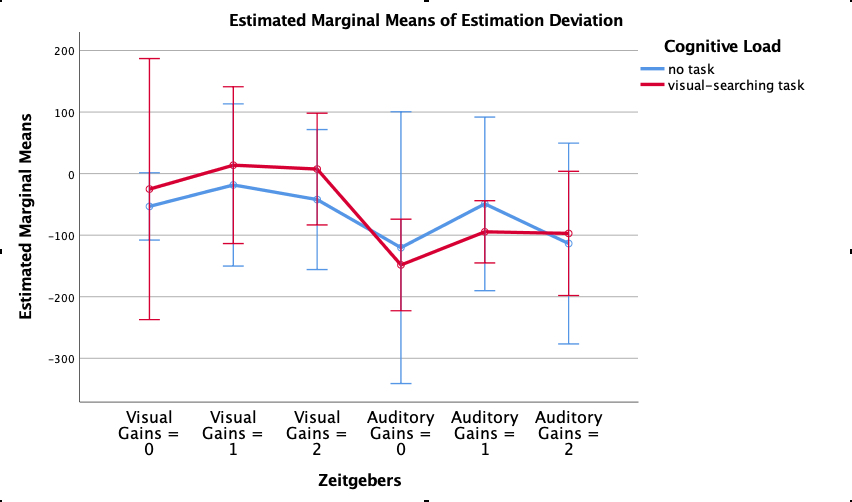
\includegraphics[width=\linewidth]{aaafiles/marginalEDZ}
%   \caption{Pooled estimated mariginal means of time estimation deviation for the comparison between different cognitive load for the different zeitgebers}
%   \label{fig:marginalEDZ}
% \end{figure}

% \begin{figure}[h]
%   \centering
%   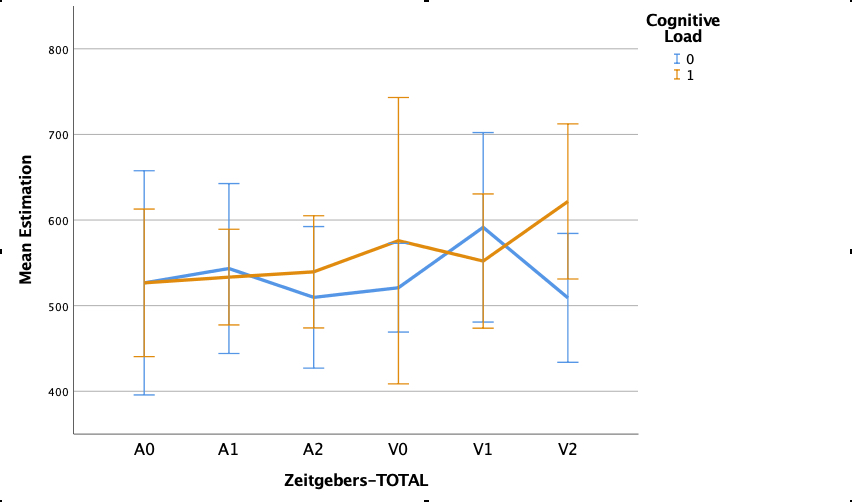
\includegraphics[width=\linewidth]{aaafiles/linezeigeberstime}
%   \caption{Pooled time estimation for the comparison between different cognitive load for the different zeitgebers}
%   \label{fig:linezeigeberstime}
% \end{figure}

Fig \ref{fig:linedeviation} shows that the mean temporal judgement deviations are different between the visual and auditory gain conditions in the IVEs, and the deviation of groups of visual gains is smaller than groups of auditory gains, which do not support our hypothesis H3. The reason of it might be that the illumination intensity was not strong enough to made our visual gains became visual zeitgebers. Besides, there are plenty of properties of light, it is possible that illumination intensity need to combine other characters of light such as color temperature to has effect on time perception.

\begin{figure}[h]
  \centering
  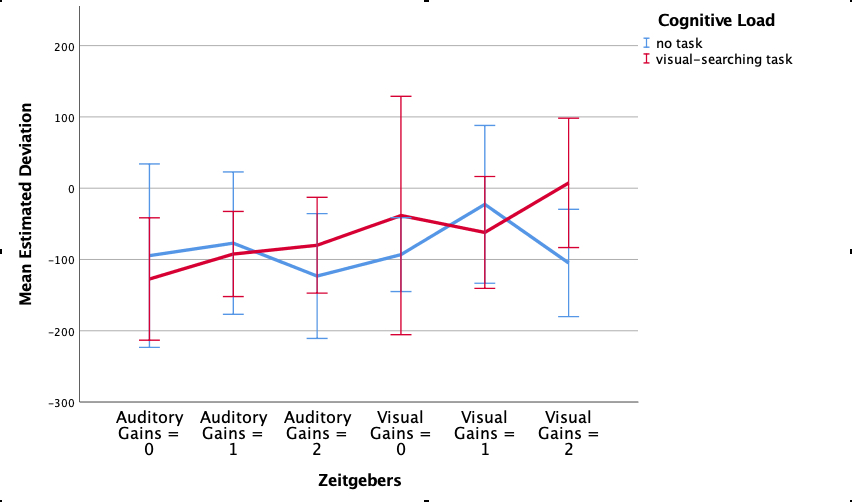
\includegraphics[width=\linewidth]{aaafiles/linedeviation}
  \caption{Pooled estimated deviation for the comparison between different cognitive load for the different zeitgebers}
  \label{fig:linedeviation}
\end{figure}

Our results show that time estimation deviation was not significantly affected by cognitive load when they immersed in VE, which do not support our hypothesis H4, although the wakening effect of task on the deviation of visual or auditory zeitgebers worked for $g_a = 2$, $g_v = 0$ and $g_v = 2$.

We found no significant main effect of immersive condition on the estimated durations deviation, and no significant effect of the difference of different immersive condition, i.e., the mean temporal judgments deviation was nearly the same between the immersive or non-immersive condition, which do not support our hypothesis H4.

To our surprise, we found a significant effect of mean skin temperature and cognitive load on time estimation in the group of visual zeitgebers when built multiple linear regression model, which indicates higher skin temperature and cognitive load will lead to bigger time estimation deviation. Besides, in line with the literature on time perception in different gender \cite{hancock1992effect}, we found the influence of gender included in the regression model on the duration estimation of participants was significant both in groups of visual or auditory zeitgebers, but in a different way. In the condition of different visual gains, male's estimated deviation is smaller than female, in groups of auditory gains, however, the opposite was true.

Our results show no significant effect of visual or auditory gains on SUS-score, and no stastic significant effect of mean SUS-score differences in different zeitgebers, which supports our hypothesis H6.

However, we found a significant simple effect of cognitive load on SUS-score when participants were immersed in VE. Besides, the differences of SUS-score between low cognitive load and high cognitive load is significant, that is, the SUS-score is lower when participants carried the visual-searching task, which do not support our hypothesis H7, and this might be due to that participants were devoted into the task when they immersed in VE and forgot about other things around them and SUS questionnaire reflected more about PI but not Psi, and a new questionnaire that take both PI and Psi into account is needed.

Furthermore, we found that there were variours factors had significant effects on SUS-score when we build the multiple linear regression model. For the group of visual gains, included gender, immersive condition, cognitive load and ITQ-score had significant effects. Although immersive condition and ITQ-score still had significant effects on SUS-score for the group of auditory gains, the other two factors became mean heart rate and mean skin temperature, which in line with the literature on the effect of physiological variables on presence \cite{meehan2002physiological,wiederhold2001investigation,sheridan1996further}.

% \section{以下为老版本}

% 采用了二因素多元方差分析方法以及多重线性回归模型对本实验的数据进行分析。

% \subsection{Zeitgebers\&CognitiveLoad-Estimation\&Presence}

% 运用两因素多元方差分析方法对授时因子和认知负载对学生时距估计和临境感的影响进行分析。

% 分析前对方法的假设进行检验:散点图发现自变量的各个组内因变量间不存在线性关系;Pearson相关发现两因变量之间不存在多重共线性($|r| < .90$);通过箱式图发现了单因素离群值, 但选择保留离群值, 通过马氏距离未发现多元离群值($p > .001$);

% Shapiro-Wilk检验显示两因变量时距估计和临境感服从正态分布($p > .05$); Box's M检验显示自变量的各个组内两个因变量的方差协方差矩阵相等($p = .047$);Levene's 检验显示各个组内时距估计方差相等($p > .05$), 但 SUS-Presence 方差相等不成立($p < .05$)。

% 授时因子和认知负载的交互作用对因变量的影响不存在统计学意义, $F = .788$, $p = .640$, $wilks'Lambda = .967$, ${\eta_p}^2 = .016$, 即授时因子对时距估计和临境感的影响在不同认知负载之间无差异。

% 多元方差分析显示授时因子对临境感的影响具有统计学意义($F = 8.138$, $p < .001$, ${\eta_p}^2 = .147$), 而对时距估计的影响不存在统计学意义($F = .327$, $p = .896$, ${\eta_p}^2 = .007$);认知负载对临境感的影响具有统计学意义($F = 13.047$, $p < .001$, ${\eta_p}^2 = .052$), 而对时距估计的影响不存在统计学意义($F = 2.052$, $p = .153$, ${\eta_p}^2 = .009$)。

% 由于授时分子是六分类变量, 因此, 对不同授时因子的临境感进行了两两比较。临境感用均值$\pm$标准差表示。授时因子为 A0, 其临境感平均值为 27.38 $\pm$ 13.406;授时因子为 A1, 其临境感平均值为 20.22 $\pm$ 12.020;授时因子为 A2, 其临境感平均值为 24.46 $\pm$ 12.353;授时因子为 V0, 其临境感平均值为 33.38 $\pm$ 10.485;授时因子为 V1, 其临境感平均值为 26.56 $\pm$ 10.961;授时因子为 V2, 其临境感平均值为 34.69 $\pm$ 10.051;

% $g_a$ = 1 组和 $g_v$ = 0 组的临境感差值为 -13.16, ($95\% CI: -20.60 - -5.72$, $p < .001$)差异具有统计学意义, $g_a$ = 1 组和 $g_v$ = 1 组的临境感差值为 -6.34, ($95\% CI: -11.67 - -1.00$, $p = .010$)差异具有统计学意义, $g_a$ = 1 组和 $g_v$ = 2 组的临境感差值为 -14.47, ($95\% CI: -21.19 - -7.03$, $p < .001$)差异具有统计学意义, $g_a$ = 2 组和 $g_v$ = 2 组的临境感差值为 -10.23, ($95\% CI: -19.44 - -1.03$, $p = .020$)差异具有统计学意义, 其余组别临境感差异均无统计学意义。

% \subsection{VRNVR\&Bio-Clock-Estimation\&Presence}

% 运用两因素多元方差分析方法对生理时钟类型和沉浸环境对参与者时距估计值和临境感的影响进行分析。

% 分析前对方法的假设进行检验:散点图发现自变量的各个组内因变量间不存在线性关系;Pearson 相关发现除了生理时钟为海豚型且在非沉浸条件下($r = -.984$)下两因变量之间存在多重共线性, 其余情况两因变量之间不存在多重共线性($|r| < .90$);通过箱式图发现了单因素离群值, 但选择保留离群值, 通过马氏距离未发现多元离群值($p > .001$);

% Shapiro-Wilk检验显示除了生理时钟类型为熊型, 且在沉浸条件下被试临境感不服从正态分布($p < .05$)外, 其余情况两因变量时距估计和临境感服从正态分布($p > .05$); Box's M检验显示自变量的各个组内两个因变量的方差协方差矩阵不相等($p < .001$);Levene's 检验显示各个组内时距估计方差不相等($p < .05$)。

% 生理时钟类型和沉浸环境的交互作用对因变量的影响不存在统计学意义, $F = .764$, $p = .549$, $Pillai's Trace = .013$, ${\eta_p}^2 = .006$, 即生理时钟类型对时距估计和临境感的影响在沉浸环境或非沉浸环境之间无差异。

% 多元方差分析显示生理时钟类型对时距估计的影响不具有统计学意义($F = .904$, $p = .406$, ${\eta_p}^2 = .007$), 对临境感的影响也不存在统计学意义($F = .030$, $p = .970$, ${\eta_p}^2 < .001$);是否为沉浸环境对临境感的影响具有统计学意义($F = 13.901$, $p < .001$, ${\eta_p}^2 = .054$), 而对时距估计的影响不存在统计学意义($F = 2.156$, $p = .143$, ${\eta_p}^2 = .009$)。

% \subsection{Zeitgebers\&Immersive Condition - Task Performance}

% 运用两因素多元方差分析方法对授时因子和沉浸条件对参与者任务表现的影响进行分析。

% 分析前对方法的假设进行检验:散点图发现自变量的各个组内因变量间不存在线性关系;Pearson 相关发现除了生理时钟为海豚型且在非沉浸条件下($r = -.984$)下两因变量之间存在多重共线性, 其余情况两因变量之间不存在多重共线性($|r| < .90$);通过箱式图发现了单因素离群值, 但选择保留离群值, 通过马氏距离未发现多元离群值($p > .001$);

% Shapiro-Wilk检验显示除了生理时钟类型为熊型, 且在沉浸条件下被试临境感不服从正态分布($p < .05$)外, 其余情况两因变量时距估计和临境感服从正态分布($p > .05$); Box's M检验显示自变量的各个组内两个因变量的方差协方差矩阵不相等($p < .001$);Levene's 检验显示各个组内时距估计方差不相等($p < .05$)。

% 生理时钟类型和沉浸环境的交互作用对因变量的影响不存在统计学意义, $F = .764$, $p = .549$, $Pillai's Trace = .013$, ${\eta_p}^2 = .006$, 即生理时钟类型对时距估计和临境感的影响在沉浸环境或非沉浸环境之间无差异。

% 多元方差分析显示生理时钟类型对时距估计的影响不具有统计学意义($F = .904$, $p = .406$, ${\eta_p}^2 = .007$), 对临境感的影响也不存在统计学意义($F = .030$, $p = .970$, ${\eta_p}^2 < .001$);是否为沉浸环境对临境感的影响具有统计学意义($F = 13.901$, $p < .001$, ${\eta_p}^2 = .054$), 而对时距估计的影响不存在统计学意义($F = 2.156$, $p = .143$, ${\eta_p}^2 = .009$)。





% %%%%%%%%%%%%%%%%%%%%%%%%%%%%%%%%%%%%% 对标论文版本



% % \subsection{Zeitgebers\&Immersive Condition-Task Performance}

% % We analyzed the effects of the different visual gains or auditory gains on visual-searching task performance in the experiment and compared the results with the baseline condition in the non-immersive setup.

% % \subsection*{Task of Visual Gains}

% % Figure \ref{} shows the differences in task performance for the immersive conditions with different visual gains and the non-immersive baseline condition with medium light intensity (i.e., $g_v$ = 1). The responses are categorized as correct responses (true positives and true negatives) as well as incorrect responses (false positives and false negatives). The results are plotted as percentages for a total of 8631 logged responses.

% % We found no significant main effect in task performance of visual group, i.e., true positives ($F = .796$, $p = .497$, ${\eta_p}^2 = .010$), true negatives ($F = .761$, $p = .517$, ${\eta_p}^2 = .009$), false positives ($F = 1.553$, $p = .201$, ${\eta_p}^2 = .019$) and false negatives ($F = .957$, $p = .414$, ${\eta_p}^2 = .012$), between the different visual gains while participants were immersed in the VE. Comparing the visual-searching task performance between the immersive and non-immersive conditions for visual gain $g_v = 1$ we found a significant difference for false positives ($F = 2.205$, $p = .139$, ${\eta_p}^2 = .009$), but not for true positives ($F = .612$, $p = .688$, ${\eta_p}^2 = .001$), true negatives ($F = .253$, $p = .616$, ${\eta_p}^2 = .001$), and false negatives ($F = .823$, $p = .365$, ${\eta_p}^2 = .003$), i.e., subjects made more errors in the immersive than in the non-immersive setup. On average, 81.64\% of the participants' responses were correct for tasks with a visual gain $g_v$ = 0, as well as 83.40\% with a visual gain $g_v$ = 1, and 84.47\% with a visual gain $g_v$ = 2. For the non-immersive condition with a visual gain $g_v$ = 1, participants' responses were correct in 86.19\% of the trials. In total, the error rates are comparably low, indicating high performance and focus of participants on this task.

% % \subsection*{Task of Auditory Gains}

% % Figure \ref{} shows the differences in task performance for the immersive conditions with different auditory gains and the non-immersive baseline condition with medium ticking speed of a clock (i.e., $g_v$ = 1). The responses are categorized as correct responses (true positives and true negatives) as well as incorrect responses (false positives and false negatives). The results are plotted as percentages for a total of 8246 logged responses.

% % We found no significant main effect in task performance of visual group, i.e., true positives ($F = .396$, $p = .756$, ${\eta_p}^2 = .005$), true negatives ($F = .137$, $p = .938$, ${\eta_p}^2 = .002$), false positives ($F = 1.227$, $p = .283$, ${\eta_p}^2 = .015$) and false negatives ($F = .179$, $p = .911$, ${\eta_p}^2 = .002$), between the different visual gains while participants were immersed in the VE. Comparing the visual-searching task performance between the immersive and non-immersive conditions for visual gain $g_v$ = 1 we found no significant difference for true positives ($F$ = .004, $p = .950$, ${\eta_p}^2 = .000$), true negatives ($F = .012$, $p = .913$, ${\eta_p}^2 = .000$), false positives ($F = .004$, $p = .949$, ${\eta_p}^2 = .000$), and false negatives ($F = .005$, $p = .942$, ${\eta_p}^2 = .000$), i.e., subjects had same performance in the immersive and in the non-immersive setup. On average, 86.22\% of the participants' responses were correct for tasks with a auditory gain $g_a$ = 0, as well as 86.93\% with a visual gain $g_a$ = 1, and 84.79\% with a visual gain $g_a$ = 2. For the non-immersive condition with a visual gain $g_a$ = 1, participants' responses were correct in 87.44\% of the trials. In total, the error rates are comparably low, indicating high performance and focus of participants on this task.





% %%%%%%%%%%%%%%%%%%%%%%%%%%%%%%%%%%%%%%%%%%%%%%%%%%%%%%%%%%%%%%%%%%%%%



% \subsection{Zeitgebers\&Cognitive Load-HR\&Skin Temperature }

% 运用两因素多元方差分析方法对授时因子和认知负载对被试各项生理指标(包括心率和皮肤温度)变化的影响进行分析。

% 分析前对方法的假设进行检验:散点图发现自变量的各个组内因变量间不存在线性关系;Pearson相关发现两因变量之间不存在多重共线性($|r| < .90$);通过箱式图发现了单因素离群值, 经分析, 其为真实的极端数据, 我们选择保留单因素离群值;通过马氏距离发现了 1 个多元离群值, 我们选择保留多元离群值;

% Shapiro-Wilk 检验显示两因变量时距估计和临境感服从正态分布($p > 0.05$); Box's M检验显示自变量的各个组内两个因变量的方差协方差矩阵相等($p = .535$);Levene's 检验显示各个组内两个因变量方差相等($p > .05$)。

% 授时因子和认知负载的交互作用对因变量的影响不存在统计学意义, $F = 1.238$, $p = .264, wilks'Lambda = .950$, ${\eta_p}^2 = .025$, 即授时因子对心率和皮肤温度的影响在不同认知负载之间无差异。

% 多元方差分析显示授时因子对心率的影响不具有统计学意义($F = .522$, $p = .760$, ${\eta_p}^2 = .011$), 对皮肤温度的影响也不存在统计学意义($F = .127$, $p = 0.986$, ${\eta_p}^2 = .003$);认知负载对心率的影响不具有统计学意义($F = 1.404$, $p = .237$, ${\eta_p}^2 = .006$), 对皮肤温度的影响也不存在统计学意义($F = .943$, $p = .333$, ${\eta_p}^2 = .004$)。

% \subsection{VRNVR\&CognitiveLoad-Estimation\&Presence
% }
% 运用两因素多元方差分析方法对沉浸条件和认知负载对参与者时距估计和临境感的影响进行分析。

% 分析前对方法的假设进行检验:散点图发现自变量的各个组内因变量间不存在线性关系;Pearson相关发现两因变量之间不存在多重共线性($|r| < .90$);通过箱式图发现了单因素离群值, 但选择保留离群值, 通过马氏距离未发现多元离群值($p > .001$);

% Shapiro-Wilk检验显示两因变量时距估计和临境感在非沉浸条件下, 无论有没有认知任务都服从正态分布($p > .05$), 但在沉浸环境没有认知任务的条件下, 只有时距估计服从正态分布($p > .05$), 而临境感不服从正态分布($p < .001$), 此外, 在沉浸环境有认知任务的条件下, 时距估计($p = .002$)和临境感都不服从正态分布($p = .005$); Box's M检验显示自变量的各个组内两个因变量的方差协方差矩阵相等($p = .383 > .001$);Levene's 检验显示各个组内时距估计和临境感方差相等($p > .05$)。

% 沉浸环境和认知负载的交互作用对因变量的影响存在统计学意义($F = 4.535$, $p = .012$, $wilks'Lambda = .964$, ${\eta_p}^2 = .036$), 即认知任务对时距估计和临境感的影响在沉浸或非沉浸环境之间存在差异。具体而言, 沉浸环境和认知负载的交互作用对临境感的影响有统计学意义($p = .003$),而对时距估计的影响不存在统计学意义($p = .867$)。

% 单因素主效应分析显示在无认知任务条件下,沉浸或非沉浸条件对时距估计的影响无统计学意义($F = .490$, $p = .485$, ${\eta_p}^2 = .002$),对临境感的影响有统计学意义($F = 41.331$, $p < .001$, ${\eta_p}^2 = .144$),在有认知任务条件下,沉浸或非沉浸条件对时距估计的影响无统计学意义($F = .217$, $p = .642$, ${\eta_p}^2 = .001$),对临境感的影响有统计学意义($F = 4.784$, $p = .030$, ${\eta_p}^2 = .019$)。而在沉浸条件下,有无认知任务对临境感的影响有统计学意义($F = 20.431$, $p < .001$, ${\eta_p}^2 = .077$),其余情况(沉浸条件下,有无认知任务对时距估计的影响 ($p = .342$) ;非沉浸条件下,有无认知任务对时距估计 ($p = .578$) 或临境感的影响 ($p = .829$) )均无统计学意义。



% % 沉浸条件对临境感的影响具有统计学意义($F = 37.229$, $p < .001$, ${\eta_p}^2 = .132$), 而对时距估计的影响不存在统计学意义($F = .681$, $p = .410$, ${\eta_p}^2 = .003$);认知负载对临境感的影响具有统计学意义($F = 7.194$, $p = .008$, ${\eta_p}^2 = .029$), $而对时距估计的影响不存在统计学意义($F = 1.068$, $p = .302$, ${\eta_p}^2 = .004$)。

% % 具体而言$, $沉浸条件无论在无认知任务($F = 41.331$, $p < .001$, ${\eta_p}^2 = .144$)或是有认知任务条件下($F = 4.784$, $p = .030$, ${\eta_p}^2 = .019$)对于临境感都有主效应$, $但认知负载对于临境感的影响只有在沉浸条件下才显著($F = 20.431$, $p < .001$, ${\eta_p}^2 = .077$)$, $在非沉浸条件下并不显著($F = .047$, $p = .829$, ${\eta_p}^2 = .000$)。

% \subsection{ALL-Estimation}

% 本研究采用多重线性回归, 根据授时因子、认知负载、VR环境、HR、ST、ITQ 和 BioClock 预测时距估计值。通过绘制部分回归散点图和学生化残差与预测值的散点图, 判断自变量和因变量之间存在线性关系。

% 已验证研究观测值之间相互独立(Durbin-Watson检验值为1.130);并通过绘制学生化残差与未标化的预测值之间的散点图, 证实数据具有等方差性。回归容忍度均大于0.1, 不存在多重共线性。异常值检验中, 存在学生化删除残差大于3倍标准差的观测值, 组别分别为5-1101, 39-0111, 42-1101。存在数据杠杆值大于0.2的组别, 分别为39-0111, 5-1101, 无Cook距离大于1的数值。Q-Q图提示, 研究数据满足正态假设。

% 回归模型不具有统计学意义 $F(12,236) = .995$, 调整 $R^2 = .048$。纳入模型的自变量对时距估计均无统计学意义($p > .05$)。

% \subsection{ALL-Presence}

% 本研究采用多重线性回归, 根据授时因子、认知负载、VR环境、HR、ST、ITQ和 BioClock 预测临境感。通过绘制部分回归散点图和学生化残差与预测值的散点图, 判断自变量和因变量之间存在线性关系。

% 已验证研究观测值之间相互独立(Durbin-Watson检验值为1.0090);并通过绘制学生化残差与未标化的预测值之间的散点图, 证实数据具有等方差性。回归容忍度均大于0.1, 不存在多重共线性。异常值检验中, 不存在学生化删除残差大于3倍标准差的观测值。不存在数据杠杆值大于0.2的组别, 无Cook距离大于1的数值。Q-Q图提示, 研究数据满足正态假设。

% 回归模型具有统计学意义$F(12,237) = 9.483$, $p < .001$, 调整$R^2 = .290$。纳入模型的部分自变量对临境感的影响具有统计学意义($p < .05$), 具体结果见表 \ref{regression}。

% \begin{table}[htbp] %表格的浮动环境
%  \centering\small
%  \begin{threeparttable}
%  \caption{Results of Multiple Linear Regression}
%  \label{regression}
%   \begin{tabular}{lccc} %表格环境,{}中是单元格对齐方式$, $l左对齐$, $c居中$, $r右对齐
%   \toprule %表头直线
%   Variables         & Coefficient & \makecell[c]{Standard\\ deviation} & \makecell[c]{Standardized\\ coefficient} \\
%   \midrule %表中直线
%   Intercept          & -46.593 & 58.510  &         \\
%   Dummy-V0          & 5.749   & 2.734   & 0.142*  \\
%   Dummy-V1          & 5.120   & 1.791   & 0.192*  \\
%   Dummy-V2          & 7.026   & 2.735   & 0.173*  \\
%   Cognitive Load    & -4.630  & 1.340   & -0.187*  \\
%   VR/NVR            & 8.095   & 1.816   & 0.321*  \\
%   Mean Heart Rate   & -0.217  & 0.087   & -0.137*  \\
%   ITQ               & 0.241   & 0.054   & 0.250*  \\
%   \bottomrule %表底直线
%  \end{tabular}
%   \small
%   % Note: Robust standard errors in parentheses. Intercept
%   %       included but not reported.
%  \begin{tablenotes}
%   \item[*] significant at 5\% level
%   % \item[**] significant at 10\% level
%  \end{tablenotes}
%  \end{threeparttable}
% \end{table}


%%%%%%%%%%%%%%%%%%%%%%%%%%%%%%%%%%%%%%%%%%%%%%%%%%%%%%%%%%%%%%%%%%%%%%%%%%%%%%

% \subsection{Time Estimation}

% \subsubsection*{Visual Gains}

% \subsubsection*{Auditory Gains}

% \subsubsection*{Cognitive Task}

% \subsubsection*{Immersion \& Presence}


% \subsection{Presence}

% \subsubsection*{Visual Gains}

% \subsubsection*{Auditory Gains}

% \subsubsection*{Cognitive Task}

% \subsection{Task Performance}

% We analyzed the effects of the different visual gains or auditory gains on visual-searching task performance in the experiment and compared the results with the baseline condition in the non-immersive setup.

% \subsection*{Task of Visual Gains}

% Figure \ref{} shows the differences in task performance for the immersive conditions with different visual gains and the non-immersive baseline condition with medium light intensity (i.e., $g_v$ = 1). The responses are categorized as correct responses (true positives and true negatives) as well as incorrect responses (false positives and false negatives). The results are plotted as percentages for a total of 8631 logged responses.

% We found no significant main effect in task performance of visual group, i.e., true positives ($F$ = .796, $p$ = .497, ${\eta_p}^2 = .010$), true negatives ($F$ = .761, $p$ = .517, ${\eta_p}^2 = .009$), false positives ($F$ = 1.553, $p$ = .201, ${\eta_p}^2 = .019$) and false negatives ($F$ = .957, $p$ = .414, ${\eta_p}^2 = .012$), between the different visual gains while participants were immersed in the VE. Comparing the visual-searching task performance between the immersive and non-immersive conditions for visual gain $g_v = 1$ we found a significant difference for false positives ($F$ = 2.205, $p$ = .139, ${\eta_p}^2 = .009$), but not for true positives ($F$ = .612, $p$ = .688, ${\eta_p}^2 = .001$), true negatives ($F$ = .253, $p$ = .616, ${\eta_p}^2 = .001$), and false negatives ($F$ = .823, $p$ = .365, ${\eta_p}^2 = .003$), i.e., subjects made more errors in the immersive than in the non-immersive setup. On average, 81.64\% of the participants' responses were correct for tasks with a visual gain $g_v$ = 0, as well as 83.40\% with a visual gain $g_v$ = 1, and 84.47\% with a visual gain $g_v$ = 2. For the non-immersive condition with a visual gain $g_v$ = 1$, $participants' responses were correct in 86.19\% of the trials. In total, the error rates are comparably low, indicating high performance and focus of participants on this task.

% \subsection*{Task of Auditory Gains}

% Figure \ref{} shows the differences in task performance for the immersive conditions with different auditory gains and the non-immersive baseline condition with medium ticking speed of a clock (i.e., $g_v$ = 1). The responses are categorized as correct responses (true positives and true negatives) as well as incorrect responses (false positives and false negatives). The results are plotted as percentages for a total of 8246 logged responses.

% We found no significant main effect in task performance of visual group, i.e., true positives ($F$ = .396, $p$ = .756, ${\eta_p}^2 = .005$), true negatives ($F$ = .137, $p$ = .938, ${\eta_p}^2 = .002$), false positives ($F$ = 1.227, $p$ = .283, ${\eta_p}^2 = .015$) and false negatives ($F$ = .179, $p$ = .911, ${\eta_p}^2 = .002$), between the different visual gains while participants were immersed in the VE. Comparing the visual-searching task performance between the immersive and non-immersive conditions for visual gain $g_v = 1$ we found no significant difference for true positives ($F$ = .004, $p$ = .950, ${\eta_p}^2 = .000$), true negatives ($F$ = .012, $p$ = .913, ${\eta_p}^2 = .000$), false positives ($F$ = .004, $p$ = .949, ${\eta_p}^2 = .000$), and false negatives ($F$ = .005, $p$ = .942, ${\eta_p}^2 = .000$), i.e., subjects had same performance in the immersive and in the non-immersive setup. On average, 86.22\% of the participants' responses were correct for tasks with a auditory gain $g_a$ = 0, as well as 86.93\% with a visual gain $g_a$ = 1, and 84.79\% with a visual gain $g_a$ = 2. For the non-immersive condition with a visual gain $g_a$ = 1$, $participants' responses were correct in 87.44\% of the trials. In total, the error rates are comparably low, indicating high performance and focus of participants on this task.

% \subsection{Physiological Variables}

% \subsubsection*{Heart Rate}

% \subsubsection*{Galvanic Skin Response}

% \subsubsection*{Skin Resistance}

% \subsubsection*{Skin Temperature}

% \subsection{Physiological Variables}

% \subsection{Questionnaires}

% ssq q h
% itq
% btq
% demo

%%%%%%%%%%%%%%%%%%%%%%%%%%%%%%%%%%%%%%%%%%%%%%%%%%%%%%%%%%%%

% Nullam mollis in lectus vitae tempus. Nam pellentesque tincidunt leo id dapibus. Etiam in euismod diam. \cite{ceres-solver, Asaro:1976:POT} Phasellus feugiat ante et dui rhoncus, at dictum elit vehicula. Nunc ut finibus neque. Sed vehicula tristique - as shown in Table \ref{soccer} - odio at interdum. Morbi ex lectus$, $porttitor vel ipsum id, scelerisque facilisis metus. Cras orci sapien, luctus in eros in, suscipit rhoncus neque. Duis pharetra elit vitae sagittis maximus. Curabitur fermentum justo massa, sed placerat odio aliquam quis. Nam facilisis hendrerit ante eget maximus. Nulla et porttitor nibh, et malesuada turpis. Suspendisse potenti. Nunc ultricies suscipit quam, eget ultrices nisi viverra vitae.

% \begin{table}[ht]
% \begin{center}
%     \caption{Soccer, or football?}
% \label{soccer}
% \begin{tabular}{l*{6}{c}r}
% Team              & P & W & D & L & F  & A & Pts \\
% \hline
% Manchester United & 6 & 4 & 0 & 2 & 10 & 5 & 12  \\
% Celtic            & 6 & 3 & 0 & 3 &  8 & 9 &  9  \\
% Benfica           & 6 & 2 & 1 & 3 &  7 & 8 &  7  \\
% FC Copenhagen     & 6 & 2 & 1 & 3 &  5 & 8 &  7  \\
% \end{tabular}
% \end{center}
% \end{table}

% Aliquam sed vehicula neque. Praesent placerat, nisi sit amet condimentum porta, justo tellus dictum eros, quis vestibulum erat massa id sapien. Vestibulum euismod purus dolor, ornare consectetur quam egestas volutpat. Curabitur sollicitudin convallis purus ultrices facilisis. Pellentesque sollicitudin maximus orci quis rutrum. Phasellus a mauris maximus sem mollis sagittis. Vivamus sagittis faucibus tincidunt. Vivamus vel suscipit leo.


% Cum sociis natoque penatibus et magnis dis parturient montes, nascetur ridiculus mus. Vivamus maximus a lectus sed dictum. Curabitur pulvinar lectus nec magna molestie consequat. Donec ligula urna, scelerisque et felis sed, euismod feugiat sem. (See equation \ref{eqn:01}.) Donec urna libero, auctor sit amet sem id, malesuada tempor risus. Morbi malesuada lobortis consequat. Aliquam lacinia quam ac tristique sodales. Class aptent taciti sociosqu ad 
% \begin{equation}
% \label{eqn:01}
% P(t)=\frac{b^{\frac{t+1}{T+1}}-b^{\frac{t}{T+1}}}{b-1},
% \end{equation}
% where $t=0,{\ldots}\,,T$, and $b$ is a number greater than $1$, litora torquent per conubia nostra$, $per inceptos himenaeos.

% \begin{multline}
% \label{the-rendering-equation}
% L_o(x, \omega_o, \lambda, t) = L_e(x, \omega_o, \lambda, t)  + \\
% \int_{\Omega} f_r(x, \omega_i, \omega_o, \lambda, t) L_i(x, \omega_i, \lambda, t)(\omega_i \cdot n) \text{d} \omega_i
% \end{multline}

% Lorem ipsum dolor sit amet, consectetur adipiscing elit. Fusce auctor accumsan nulla, vitae pharetra ipsum sagittis sit amet. Donec ac metus consectetur, venenatis magna sit amet, viverra sapien. Class aptent taciti sociosqu ad litora torquent per conubia nostra$, $per inceptos himenaeos. Phasellus eleifend sem sit amet arcu congue tempus. Proin at iaculis orci. (See equation \ref{the-rendering-equation}.) Pellentesque habitant morbi tristique senectus et netus et malesuada fames ac turpis egestas. Orci varius natoque penatibus et magnis dis parturient montes, nascetur ridiculus mus. Etiam feugiat dui sit amet ante pellentesque, sed malesuada libero ornare. Curabitur tempor ligula leo, in feugiat urna ornare luctus. Fusce quis metus sit amet neque sagittis elementum. Quisque facilisis quam quis tortor volutpat, et sodales urna efficitur.

\section{Conclusions and Future Work}

% Nullam vulputate enim ut tortor mollis pharetra. Cras pellentesque sem a accumsan malesuada. Donec at massa nisl. Sed malesuada felis id nisl maximus efficitur. In pretium metus non faucibus pulvinar. Sed pulvinar elit ultrices mauris vehicula, id ultricies purus finibus. Fusce tempus elit molestie, consequat ipsum eget, iaculis nibh. Cras tincidunt, orci in lacinia tempus, mauris leo finibus orci, vitae dignissim dui risus et odio. Sed commodo ultricies nulla, et varius velit aliquam quis. Sed efficitur, ex non facilisis dignissim, lacus orci accumsan massa, dictum facilisis arcu lacus ac leo. Sed quis tellus dictum massa egestas dapibus vel et justo. Nulla euismod lectus ut purus hendrerit porttitor. Suspendisse quis dui ligula. Proin non porta libero. Maecenas vel feugiat urna.

In this article, we further explored the effects of manipulated visual or auditory zeitgebers, cognitived load and immersion on time estimation and presence as yet not well-studied factors of spatiotemporal perception and presence perception in VEs. We presented an experiment in which we analyzed the ability of temporal perception and sence of presence while experiencing an immersive HMD as well as non-immersive VE. 

We found a significant effect of skin temperature on time estimation when participants were in different groups of visual zeitgebres, which indicates that people with higher skin temperature may have better time perception in a way, and this provide a guideline for the build of time-passing virtual environment. Besides, we found a significant effect of gender on time estimation in group of visual or auditory zeitgebers, but in a different way, i.e., male has better judgement for time than female in the group of visual zeitgebers, and female has better temporal perception than male in the group of auditory zetgebers. This suggests that we need to take gender into account when building time-related applications in order to influence users' perception of time better. Moreover, due to the limitation of SUS questionnaire, we think a new questionnaire which can take both PI and Psi into account is needed.

Higher cognitive load might lead to lower SUS-score, which provide a guidence that if we want the participants feel more place illusion, we need to ovoid overinvolving the user in their task. Not only cognitive load had significant influence on SUS-score, gender, immersive condition, and ITQ-score were also influencial in group of visual zeitgebers, immersive condition, ITQ-score, mean heart rate and mean skin temperature had significant effects on SUS-score in group of auditory zeitgebers, which could guide us to build more attracted computer-generated virtual worlds.

In the future, we plan to investigate zeitgebers with much bigger discrimination and influencial on time perception. For visual zeitgebers, we plan to take the different characters of light into acount, such as color temperature and wave length. Futhermore, we plan to investigate alternative zeitgebers such as sound of wind or rain incorporating also multimodal information such as environment temperature. Besides, we want to build more interactive and reliable scenarios, for instance, in which users can have conversation with other creature so the social zeitgebers can be take into acount.

With the advent of 5G era, apparently, VR technology will play a bigger role in the near future, and it is important to figure out how time is perceived and the sence of presence in VR. This research provides a new perspective towards understanding temporal perception and sence of presence in IVEs, and we believe that the potential of this topic will attract people to join us and explore the principles behind perceiving and even manipulating time in virtual reality environments.


\begin{acks}
% The authors would like to thank Dr. Yuhua Li for providing the MATLAB code of the \textit{BEPS} method.
% The authors would also like to thank the anonymous referees for their valuable comments and helpful suggestions. The work is supported by the \grantsponsor{GS501100001809}{National Natural Science Foundation of China}{https://doi.org/10.13039/501100001809} under Grant No.: ~\grantnum{GS501100001809}{61273304}
% 21 and ~\grantnum[http://www.nnsf.cn/youngscientists]{GS501100001809}{Young Scientists' Support Program}.
\end{acks}

\bibliographystyle{ACM-Reference-Format}
\bibliography{aaatemplate}

\end{document}